\graphicspath{{main/chapter3/fig/}}

\chapter{Optimization Strategies}

% \vspace*{\fill}
\minitoccustom
% \vspace*{\fill}

% \section{Algorithmic Simplifications}

% \section{Memory Data Layer}

% \section{Quantification}

% \section{Vectorization~\cite{Cassagne2018}}

\section{\MIPP: A \Cxx Wrapper for SIMD Instructions}

Recent articles have proposed several optimized software decoders, corresponding
to different channel codes : LDPC codes~\cite{LeGal2015,LeGal2016}, polar
codes~\cite{Giard2016b,Sarkis2016,Cassagne2015c,Cassagne2016b}, turbo
codes~\cite{Zhang2012,Wu2013,Cassagne2016a}. All of these works show the
possibility to reach a good level of \textit{performance} by  making extensive
use of SIMD (Single Instruction Multiple Data) units. This is often achieved at
the price of a reduced \textit{flexibility}, by resorting to specific
intrinsics, or by making assumptions on the data types. However, these decoders
should be implemented in a single source code, in which the following parameters
could be changed at runtime: the channel code type, the decoding algorithm, the
number of decoding iterations, the data format, etc. Another important aspect is
the \textit{portability} of the source code on different hardwares (Intel\R x86,
Xeon Phi\TM KNL and ARM\R) and the possibility to use different instruction sets
(SSE, AVX, AVX-512, NEON). These three constraints (performance, flexibility,
portability) push towards the use of a SIMD library that helps in the
abstraction of the SIMD instruction sets, while still allowing a fine grain
tuning of performance.

We propose in this thesis a new \Cxx SIMD wrapper, covering the needs in terms
of expressiveness and of performance for the channel codes. Our contributions
are:
\begin{itemize}
  \item A portable and high performance  \Cxx SIMD wrapper called \MIPP, for
    SSE, AVX, AVX-512 and NEON instruction sets;
  \item An implementation of several channel codes with this wrapper. We
    present the main advantages of \MIPP in this context;
  \item A comparison with other state-of-the-art SIMD wrappers on a Mandelbrot
    code, demonstrating that the code based on \MIPP has similar performance as
    hand-written intrinsics.
\end{itemize}
\MIPP programming model is not too far from intrinsics, allowing a good control
on performance, but still provides an abstraction on the basic types used in
vectors (ranging from double to byte) and complex operations (parametric
reductions, log, exponential, ...).

The \longMIPP library (\MIPP) is a portable wrapper for SIMD intrinsics written
in the \Cxx language. It relies on \Cxx compile-time template specialization
techniques to replace supported generic functions with inline calls to their
intrinsics counterpart, for a given instruction set. While \MIPP is mostly
written in \Cxy{98}, it still requires \Cxy{11}-compliant compiler due to the
use of convenient features such as the \verb|auto| and \verb|using| keywords.
\MIPP is Open-source (under the MIT license) and the full code is available on
GitHub\footnote{\MIPP source code: \url{https://github.com/aff3ct/MIPP}}.

\MIPP provides two application programming interface levels. The
\emph{Low Level Interface} (low) implements a basic, thin abstraction layer on
top of the intrinsics. The \emph{Medium Level Interface} (med.), built on top of
\MIPP low, abstracts away more details to lessen the effort from the application
programmer by relying on object encapsulation and operator overloading.

\subsection{Low Level Interface}

\MIPP low is built around a unified \verb|mipp::reg| type that abstracts vector
registers. The vector register type represents hardware registers independently
of the data type of the vector elements. \MIPP uses the longest native vector
length available on the architecture. This design choice preserves programmer
flexibility, for instance in situations such as mixing fixed-point and
floating-point operations. \MIPP also defines a \emph{mask} register type
\verb|mipp::msk|, which either directly maps to real hardware masks on
instruction sets that support it (such as AVX-512), or to simple vector
registers otherwise.

\MIPP low then defines a set of functions working with \verb|mipp::reg| and
\verb|mipp::msk|, organized into eight families: memory accesses, shuffles,
bitwise boolean arithmetic, integer operations, float. operations, mathematical
functions, reductions, and mask operations.

In the AVX-512 instruction set, one \textit{regular} vector operation plus one
masking operation can be performed in one CPU clock cycle. For instance, the
following instruction performs \verb|"m ? a+b : src"|, an addition and a masking
operation:
\mint{C++}|__m512 _mm512_mask_add_ps(__m512 src, __mmask16 m, __m512 a, __m512 b);|

\MIPP natively supports such operations with the \verb|mipp::mask| function. The
previous example becomes in \MIPP:
\mint{C++}|mipp::mask<float,mipp::add<float>>(m, src, a, b);|
For instruction sets without masking support, the \verb|mipp::mask| call is
expanded as an operation and a \verb|blend| instead.

\subsection{Medium Level Interface}

\begin{listing}[htp]
  \inputminted[frame=lines,linenos]{C++}{main/chapter3/src/mipp/mli.cpp}
  \caption{Medium Level Interface encapsulation.}
  \label{lst:vec_mipp_mli}
\end{listing}

The \MIPP Medium Level Interface (\MIPP med.) provides additional expressiveness
to the programmer. \verb|mipp::reg| and \verb|mipp::msk| basic types are
encapsulated in \verb|mipp::Reg<T>| and \verb|mipp::Msk<N>| objects,
respectively. The \verb|T| and \verb|N| template parameters correspond to the
type and the number of elements inside the vector register and the mask
register, respectively. One can notice that in these register objects are typed,
unlike the \MIPP low register basic type. It avoids to write the type when a
\MIPP function is called. The function type can then be directly selected from
the parameter type. Listing~\ref{lst:vec_mipp_mli} illustrates the
template-based encapsulation, which enables \MIPP to override common arithmetic
and comparison operators.

\MIPP med. also simplifies register loading and initialization operations. The
constructor of the \verb|mipp::Reg| object will call the \verb|mipp::load|
function automatically. Thus, a load in \MIPP low:
\mint{C++}|mipp::reg a = mipp::load<float>(aligned_ptr);|
can be simplified into:
\mint{C++}|mipp::Reg<float> a = aligned_ptr;|
with \MIPP med. level. An initializer list
can be used with a \MIPP med. vector register:
\mint{C++}|mipp::Reg<float> a = {1.f, 2.f, 3.f, 4.f};|
Likewise, a scalar assigned to a vector sets all elements to
this value.

\subsection{Implementation Details}
\label{sec:vec_mipp_implem}

\MIPP targets SSE2, SSE3, SSSE3, SSE4.1, SSE4.2, AVX, AVX2, FMA3, KNCI, AVX-512F
and AVX-512BW instruction sets on x86 and related architectures, as well as
NEON, NEONv2, NEON64 and NEON64v2 on ARM\R. It can easily be extended to other
instruction sets.

\MIPP selects the most recent instruction set available at compile time. For
instance, a code compiled with the \verb|-march=avx| flag of the GNU GCC
compiler uses \verb|AVX| instructions even if the architecture supports
\verb|SSE| as well. The vector register size is determined by the instruction
set and the data type. A dedicated function returns the number of elements in a
\MIPP register:
\mint{C++}|constexpr int n = mipp::nElmtsPerRegister<T>();|
A shortened version is also defined as: \verb|mipp::N<T>()|. Whenever
vectorization takes place in loops, \MIPP's philosophy is to change the stride
of the loop from one to the size of registers. The stride can be statically
determined with the \verb|mipp::N<T>()| function.
If the loop size is not a multiple of the registers size, 1) a sequential tail
loop can be implemented to compute the remaining elements, 2) the padding
technique can be implemented to force the loop size to be a multiple of the
vector registers.

When the instruction set cannot be determined, \MIPP med. falls back on
sequential instructions. In this case, \MIPP does not use any intrinsic anymore.
However, the compiler vectorizer still remains effective. This mode can also be
selected by the programmer with the \verb|MIPP_NO_INTRINSICS| macro.

\MIPP supports the following data types: \verb|double|, \verb|float|,
\verb|int64_t|, \verb|int32_t|, \verb|int16_t| and \verb|int8_t|. It also
supplies an aligned memory allocator, to be used with types such as the
\verb|std::vector<T,A>| vector container from the \Cxx standard library (where
\verb|T| is the vector element type and \verb|A| the allocator). The alignment
requirements are not guaranteed by the default \Cxx memory allocator. The \MIPP
memory allocator can be used as follows:
\mint{C++}|std::vector<T,mipp::allocator> aligned_data;|
and shortened like this: \verb|mipp::vector<T>|.

\MIPP comes with a comprehensive unitary test suite to validate new instruction
set ports and new feature implementations. It has successfully been tested with
the following minimum compiler versions: \verb|g++-4.8|, \verb|clang++-3.6|,
\verb|icpc15| and \verb|msvc14.0|.

\MIPP implements a generic reduction operator based on a reduction tree, which
would be tedious to write by the application programmer, due to the sequence of
heterogeneous shuffle instructions it implies. The computational complexity of
this algorithm is $O(\log_2(N))$, with $N$ the number of elements in a register.
It can operate on \verb|mipp::reg|, \verb|mipp::Reg<T>| and
\verb|std::vector<T>|. It can also work on dynamically allocated arrays,
provided the length of the array is a multiple of the vector register size.
Since the function passed to the reduction operator is resolved at the compile
time, the code remains efficient. Any function with the following prototype can
be used as the reduction function:
\mint{C++}|mipp::Reg<T> func(mipp::Reg<T>, mipp::Reg<T>);|
E.g., the code below computes the smallest element in a register:
\begin{minted}{C++}
mipp::Reg<float> r = {4.f, 2.f, 1.f, 3.f};
float min = mipp::Reduction<mipp::min>::sapply(r);
\end{minted}
The \verb|min| scalar variable will be assigned \verb|1.f| as the result. For
convenience, a set of functions is predefined, based on this generic reduction
feature: \verb|hadd|, \verb|hsub|, \verb|hmul| and \verb|hdiv|.

\subsection{Experimentation Protocol}

\begin{table}[htp]
  \tabcolsep=6pt
  \centering
  \caption{Specifications of the target processors.}
  \label{tab:vec_specs}
  % {\small\resizebox{\linewidth}{!}{
  \begin{tabular}{c | c c c c}
  \textbf{Name}                   & \textbf{Exynos5422} & \textbf{RK3399} & \textbf{Core\TM i5-5300U}  & \textbf{Xeon Phi\TM 7230} \\ \hline \hline
  \textbf{Year}                   & 2014                & 2016            & 2015                       & 2016                      \\ %\hline
  \textbf{Vendor}                 & Samsung\R           & Rockchip\R      & Intel\R                    & Intel\R                   \\ %\hline
  \multirow{2}{*}{\textbf{Arch.}} & ARMv7               & ARMv8           & \multirow{2}{*}{Broadwell} & Knights                   \\
                                  & Cortex-A15          & Cortex-A72      &                            & Landing                   \\ %\hline
  \textbf{Cores/Freq.}            & 4/2.0 GHz           & 2/1.6 GHz       & 2/2.3 GHz                  & 64/1.3 GHz                \\ %\hline
  \textbf{LLC}                    & 2 MB L2             & 1 MB L2         & 3 MB L3                    & 32MB L2                   \\ %\hline
  \textbf{TDP}                    & $\sim$4 W           & $\sim$2 W       & 15 W                       & 215 W                     \\
  \end{tabular}
  % }}
\end{table}

Four architectures are considered for performance results, summarized in
Table~\ref{tab:vec_specs}. The Cortex-A15 is used to evaluate the NEON
instruction set in 32-bit. The Cortex-A72 is used to evaluate the 64-bit NEON
instructions for Figure~\ref{plot:vec_mandelbrot}. The Core\TM i5 is used for
both SSE and AVX benchmarks. The Xeon Phi\TM is used for AVX-512 instructions.
Source codes are compiled with the GNU \Cxx~5 compiler using the common flags:
\verb|-O3| \verb|-funroll-loops|. The additional architecture specific flags
are:
1) \verb|-march=armv7-a| \verb|-mfpu=neon-vfpv4| on Cortex-A15,
2) \verb|-march=armv8-a| on Cortex-A72,
3) \verb|-msse4.2| for SSE or \verb|-mavx2 -mfma| for AVX on Core\TM i5,
4) \verb|-mavx512f| \verb|-mfma| on Xeon Phi\TM.
All experiments have been performed in single-threaded. All studied problem
sizes fit into the last level cache (LLC) of CPUs. The references for the
speedup computations are always sequential versions of the SIMD codes. Those
reference versions can be auto-vectorized by the compiler, thus a reference
version is compiled for each SIMD instruction set.

\subsection{Related Works}

Many SIMD programming solutions have been surveyed in~\cite{Pohl2016} to take
advantage of modern instruction sets. The existing alternatives can be
decomposed into three main models: 1)~intrinsics or assembly code; 2)~dedicated
language; and 3)~dedicated library. The intrinsics or assembly approaches are
non-portable, low-level solutions which target specific architectures. They
offer maximum control to take advantage of instruction set specificities, and to
fine tune register usage. However, it is quite difficult to develop and maintain
a low-level code in the long run. Some languages have been designed to provide
programmers with SIMD programming constructs. Many of them are based on general
purpose languages extended with some kinds of annotation mechanism (e.g.
pragmas) such as OpenMP~\cite{OpenMP2013}, Cilk Plus~\cite{Robison2013} or
ispc~\cite{Pharr2012}. They offer higher expressiveness, better portability and
generally more readable code, at the expense of less programmer control, and
vectorization performance. More specialized languages, such as
OpenCL~\cite{Howes2015}, enable the programmer to retain more control, as the
counterpart of writing some more specific code.
In this paper, the focus is given to the library approach since we want to
maximize performance, maximize portability and deal with existing \Cxx codes. In
order to let the compiler inline library calls, which is critical for the
intended SIMD programming model purpose, such library are usually header-only.
Thus, we refer to them as \textit{wrappers} instead of \textit{libraries}.

\subsubsection{\Cxx SIMD Wrappers}

\begin{itemize}
  \item \xmark~mettre à jour les wrappers SIMD, il y en a de nouveaux et les
    actuels ont évolués
  \item \xmark~problème: il faudrait refaire les XP
    Figure~\ref{plot:vec_mandelbrot} et tout le discours qui va avec... :-(
    (solution possible : citer et dater l'article pour dire de quand date la
    mise à jour)
\end{itemize}

% \begin{table}
%   \renewcommand{\arraystretch}{0.95}
%   \tabcolsep=6pt
%   \centering
%   \caption{Comparison of various SIMD wrappers.}
%   \label{tab:vec_comparison}
%   \begin{adjustbox}{angle=90}
%   {\resizebox{0.975\textheight}{!}{
%   \begin{tabular}{|r|r|r|r|r||c|c|c|c|c||c|c|c|c|c|c||c|c|c|}
%   \hline
%   \multicolumn{5}{|c||}{\multirow{2}{*}{\textbf{General Information}}}                                                               & \multicolumn{5}{c||}{\multirow{2}{*}{\textbf{Instruction Set}}}                                                                & \multicolumn{6}{c||}{\multirow{2}{*}{\textbf{Data Type}}}                    & \multicolumn{3}{c|}{\multirow{2}{*}{\textbf{Features}}} \\
%   \multicolumn{5}{|c||}{}                                                                                                            & \multicolumn{5}{c||}{}                                                                                                         & \multicolumn{6}{c||}{}                                                       & \multicolumn{3}{c|}{}                                  \\ \hline
%   \multicolumn{2}{|r|}{\textbf{Name}}                                      & \textbf{Ref.}       & \textbf{Start} & \textbf{License} & \textbf{SSE} & \textbf{AVX} & \textbf{AVX-512} & \textbf{NEON} & \textbf{AltiVec} & \multicolumn{2}{c|}{\textbf{Float}} & \multicolumn{4}{c||}{\textbf{Integer}} & \textbf{Math}  & \textbf{\Cxx}      & \textbf{Test}    \\ \cline{11-16}
%   \multicolumn{2}{|r|}{}                                                   &                     & \textbf{Year}  &                  & 128-bit      & 256-bit      & 512-bit          & 128-bit       & 128-bit          & 64      & 32                        & 64     & 32     & 16     & 8           & \textbf{Func.} & \textbf{Technique} & \textbf{Suite}   \\ \hline \hline
%   \multirow{8}{*}{\rotatebox[origin=c]{90}{\textbf{Library}}} & \MIPP      & $-$                 & 2013           & MIT              & \cmark       & \cmark       & \cmark           & \cmark        & \xmark           & \cmark  & \cmark                    & \cmark & \cmark & \cmark & \cmark      & \cmark         & Op. overload.      & \cmark           \\ \cline{2-19}
%                                                               & \VCL       & \cite{Fog}          & 2012           & GNU GPL          & \cmark       & \cmark       & \cmark           & \xmark        & \xmark           & \cmark  & \cmark                    & \cmark & \cmark & \cmark & \cmark      & \cmark         & Op. overload.      & \textbf{N/A}     \\ \cline{2-19}
%                                                               & \simdpp    & \cite{Kanapickas}   & 2013           & Boost Software   & \cmark       & \cmark       & \cmark           & \cmark        & \cmark           & \cmark  & \cmark                    & \cmark & \cmark & \cmark & \cmark      & \xmark         & Expr. templ.       & \cmark           \\ \cline{2-19}
%                                                               & \TSIMD     & \cite{Moller2016}   & 2016           & Open-source      & \cmark       & \cmark       & \xmark           & \cmark        & \xmark           & \xmark  & \cmark                    & \xmark & \cmark & \cmark & \cmark      & \xmark         & Op. overload.      & \textbf{N/A}     \\ \cline{2-19}
%                                                               & \Vc        & \cite{Kretz2012}    & 2012           & BSD-3-Clause     & \cmark       & \cmark       & \xmark           & \xmark        & \xmark           & \cmark  & \cmark                    & \cmark & \cmark & \cmark & \xmark      & \cmark         & Op. overload.      & \cmark           \\ \cline{2-19}
%                                                               & \xsimd     & \cite{Mabille}      & 2014           & BSD-3-Clause     & \cmark       & \cmark       & \xmark           & \xmark        & \xmark           & \cmark  & \cmark                    & \cmark & \cmark & \xmark & \xmark      & \cmark         & Op. overload.      & \textbf{N/A}     \\ \cline{2-19}
%                                                               & \BoostSIMD & \cite{Esterie2012}  & 2012           & Boost Software   & \cmark       & \xmark       & \xmark           & \xmark        & \xmark           & \cmark  & \cmark                    & \cmark & \cmark & \cmark & \cmark      & \cmark         & Expr. templ.       & \cmark           \\ \cline{2-19}
%                                                               & \bSIMD     & \cite{Esterie2012a} & 2017           & Non-free         & \cmark       & \cmark       & \cmark           & \cmark        & \cmark           & \cmark  & \cmark                    & \cmark & \cmark & \cmark & \cmark      & \cmark         & Expr. templ.       & \cmark           \\ \hline
%   \end{tabular}
%   }}
%   \end{adjustbox}
% \end{table}

\begin{table}[htp]
  % \renewcommand{\arraystretch}{0.95}
  % \tabcolsep=6pt
  \centering
  \caption{Comparison of various SIMD wrappers: General Information and Features.}
  \label{tab:vec_comparison}
  % \begin{adjustbox}{angle=90}
  % {\resizebox{\linewidth}{!}{
  \begin{tabular}{r r r r | c c c}
  % \hline
  \multicolumn{4}{c|}{\multirow{2}{*}{\textbf{General Information}}}      & \multicolumn{3}{c}{\multirow{2}{*}{\textbf{Features}}}\\
                &                     &                &                  &                &                    &                 \\ \hline
  \textbf{Name} & \textbf{Ref.}       & \textbf{Start} & \textbf{License} & \textbf{Math}  & \textbf{\Cxx}      & \textbf{Test}   \\ %\cline{11-16}
                &                     & \textbf{Year}  &                  & \textbf{Func.} & \textbf{Technique} & \textbf{Suite}  \\ \hline \hline
  \MIPP         & \cite{Cassagne2018} & 2013           & MIT              & \cmark         & Op. overload.      & \cmark          \\ %\cline{2-19}
  \VCL          & \cite{Fog}          & 2012           & GNU GPL          & \cmark         & Op. overload.      & \textbf{N/A}    \\ %\cline{2-19}
  \simdpp       & \cite{Kanapickas}   & 2013           & Boost Software   & \xmark         & Expr. templ.       & \cmark          \\ %\cline{2-19}
  \TSIMD        & \cite{Moller2016}   & 2016           & Open-source      & \xmark         & Op. overload.      & \textbf{N/A}    \\ %\cline{2-19}
  \Vc           & \cite{Kretz2012}    & 2012           & BSD-3-Clause     & \cmark         & Op. overload.      & \cmark          \\ %\cline{2-19}
  \xsimd        & \cite{Mabille}      & 2014           & BSD-3-Clause     & \cmark         & Op. overload.      & \textbf{N/A}    \\ %\cline{2-19}
  \BoostSIMD    & \cite{Esterie2012}  & 2012           & Boost Software   & \cmark         & Expr. templ.       & \cmark          \\ %\cline{2-19}
  \bSIMD        & \cite{Esterie2012a} & 2017           & Non-free         & \cmark         & Expr. templ.       & \cmark          \\ %\hline
  \end{tabular}
  % }}
  % \end{adjustbox}
\end{table}


\begin{table}[htp]
  % \renewcommand{\arraystretch}{0.95}
  % \tabcolsep=6pt
  \centering
  \caption{Comparison of various SIMD wrappers : Supported ISA and Data Type.}
  \label{tab:vec_comparison}
  % \begin{adjustbox}{angle=90}
  % {\resizebox{\linewidth}{!}{
  \begin{tabular}{r || c c c c c || c c | c c c c}
  % \hline
  {\multirow{4}{*}{\textbf{Name}}} & \multicolumn{5}{c||}{\multirow{2}{*}{\textbf{Instruction Set}}}                 & \multicolumn{6}{c}{\multirow{2}{*}{\textbf{Data Type}}}                    \\
                                   & \multicolumn{5}{c||}{}                                                          & \multicolumn{6}{c}{}                                                       \\ \cline{2-12}
                                   & \textbf{SSE} & \textbf{AVX} & \textbf{AVX512} & \textbf{NEON} & \textbf{AltiV.} & \multicolumn{2}{c|}{\textbf{Float}} & \multicolumn{4}{c}{\textbf{Integer}} \\ %\cline{2-12}
                                   & 128-bit      & 256-bit      & 512-bit         & 128-bit       & 128-bit         & 64      & 32                        & 64     & 32     & 16     & 8         \\ \hline \hline
  \MIPP                            & \cmark       & \cmark       & \cmark          & \cmark        & \xmark          & \cmark  & \cmark                    & \cmark & \cmark & \cmark & \cmark    \\ %\cline{2-19}
  \VCL                             & \cmark       & \cmark       & \cmark          & \xmark        & \xmark          & \cmark  & \cmark                    & \cmark & \cmark & \cmark & \cmark    \\ %\cline{2-19}
  \simdpp                          & \cmark       & \cmark       & \cmark          & \cmark        & \cmark          & \cmark  & \cmark                    & \cmark & \cmark & \cmark & \cmark    \\ %\cline{2-19}
  \TSIMD                           & \cmark       & \cmark       & \xmark          & \cmark        & \xmark          & \xmark  & \cmark                    & \xmark & \cmark & \cmark & \cmark    \\ %\cline{2-19}
  \Vc                              & \cmark       & \cmark       & \xmark          & \xmark        & \xmark          & \cmark  & \cmark                    & \cmark & \cmark & \cmark & \xmark    \\ %\cline{2-19}
  \xsimd                           & \cmark       & \cmark       & \xmark          & \xmark        & \xmark          & \cmark  & \cmark                    & \cmark & \cmark & \xmark & \xmark    \\ %\cline{2-19}
  \BoostSIMD                       & \cmark       & \xmark       & \xmark          & \xmark        & \xmark          & \cmark  & \cmark                    & \cmark & \cmark & \cmark & \cmark    \\ %\cline{2-19}
  \bSIMD                           & \cmark       & \cmark       & \cmark          & \cmark        & \cmark          & \cmark  & \cmark                    & \cmark & \cmark & \cmark & \cmark    \\ %\hline
  \end{tabular}
  % }}
  % \end{adjustbox}
\end{table}

Table~\ref{tab:vec_comparison} compares various SIMD wrappers. It aims to
present an overview of some prominent solutions, though it is by no means
exhaustive due to the richness of the SIMD wrapper landscape. Some of the
wrappers presented, such as \MIPP, \Vc, \BoostSIMD, \VCL and \TSIMD, have been
designed in an academic research context. Some others, \simdpp and \xsimd,
appear to be standalone development efforts by individual programmers or
maintainers. Proprietary, closed-source solutions also exist on the market, such
as \bSIMD, which is an extended version of \BoostSIMD, or the commercial version
of \VCL. The \textit{Instruction Set} column is broken up into five families
among the most widely available on the market: NEON, SSE, AVX, AVX-512 and
AltiVec. For the sake of conciseness, we choose not to list all the instruction
sets ``sub-variants'' (such as SSE2, SSE3, etc). \simdpp et \bSIMD propose the
most comprehensive instruction set compatibility. At the other end of the range,
\xsimd and \BoostSIMD only support Intel\R SIMD instruction sets. The
\textit{Data Type} column of the table summarizes the supported vector element
types and precisions. In their public version, and at the time of writing, \Vc
does not support 8-bit integers, \xsimd does not support 8-bit and 16-bit
integers and \TSIMD does not support 64-bit data types, to the best of our
knowledge. The \textit{Features} column highlights some additional
characteristics. The \textit{Math Func.}~ column indicates which wrapper
supports additional mathematical sub-routines, not necessarily available as
native CPU instructions (exponential, logarithm, trigonometric functions for
instance), and required by algorithms such as the Box-Muller Transform (see
Section~\ref{sec:vec_awgn}). The \textit{\Cxx Technique} column indicates
whether the wrapper is designed as an expression template framework, or whether
it relies on operator overloading techniques. The expression template feature is
a powerful technique to automatically drive the rewriting of whole arithmetic
expressions into SIMD hardware instructions or instruction sequences. For
instance if the user writes \verb|d = a * b + c|, the wrapper can automatically
match a \emph{fused multiply and add} instruction (FMA). \BoostSIMD and \bSIMD
extensively use this technique~\cite{Esterie2012,Esterie2012a}. The drawbacks
are that the source code complexity of the wrapper is dramatically increased.
\BoostSIMD and \bSIMD have a dependency on the Boost framework to build, and
currently available \Cxx compilers produce huge amounts of arcane error messages
at the slightest mistake in the end user program. For these reasons, we decided
not to base \MIPP on the expression template technique. As mentioned in
Section~\ref{sec:vec_mipp_implem}, maintaining SIMD wrappers, and porting them
to new instruction sets is error prone by nature, due to the large number of
routines, cryptic intrinsics names, and specific instruction set details. A
comprehensive testing suite is therefore critical to validate new development,
optimizations and ports on new instruction sets. This is why \MIPP, as well as
\Vc, \BoostSIMD, \simdpp and \bSIMD come with their own test suites. We have not
found similar test suites in the software distributions of \VCL, \xsimd and
\TSIMD; however, test suites might be in use internally, within the development
teams of these wrappers.

\subsubsection{Qualitative and Quantitative Comparisons}

\begin{figure}[htp]
  \centering
  \subfloat[][Float 32-bit]{\includegraphics[width=0.485\textwidth]{vectorization/mandelbrot_speedup/mandelbrot_speedup_32bit}\label{plot:vec_mandelbrot_32}}
  \quad
  \subfloat[][Float 64-bit]{\includegraphics[width=0.485\textwidth]{vectorization/mandelbrot_speedup/mandelbrot_speedup_64bit}\label{plot:vec_mandelbrot_64}}
  \caption{Speedups over the Mandelbrot naive auto-vectorized implementation.}
  \label{plot:vec_mandelbrot}
\end{figure}

We now compare \MIPP with the open-source wrappers presented above, both
qualitatively for our error correction code purpose, and quantitatively on a
well known benchmark the computation of the Mandelbrot set, to prevent as much
as possible the risk of unfairness of the port on each wrapper. This problem is
compute-bound. The chosen implementation relies on a floating-point
representation (available online\footnote{Mandelbrot set source code:
\url{https://gitlab.inria.fr/acassagn/mandelbrot}}).
Figure~\ref{plot:vec_mandelbrot} presents the speedups obtained on various
instruction sets on single-precision floating-point format (cf.
Fig.~\ref{plot:vec_mandelbrot_32}) and on double-precision floating-point format
(cf. Fig.~\ref{plot:vec_mandelbrot_64}). SSE stands for SSE4.2, NEON stands for
NEONv2 (includes the FMA instructions), AVX stands for AVX2+FMA3 and AVX-512
stands for AVX-512F (with FMA instructions). The FMA benefit ranges from 17\%
(AVX2) to 26\% (AVX-512). An SIMD with intrinsics version has been hand-coded
for each specific instruction set. The intrinsics version is considered the
``\emph{golden}'' model.

\textbf{\BoostSIMD} only supports the SSE instruction set, even when the code is
compiled with one of the AVX or AVX-512 flags. It is insufficient for our
channel coding processing purpose. The \BoostSIMD wrapper performance results
that were obtained are disappointing. The sequential Mandelbrot kernel does an
early exit in the innermost loop, as soon as the divergence of the sequence is
detected for the input coordinates. We were unable to SIMDize this early
termination with \BoostSIMD, because the \verb|boost::simd::any| function was
not available in the GitHub repository at the time of writing. \textbf{\xsimd}
achieves performance close to the intrinsic version in SSE and AVX. However, it
currently lacks NEON and AVX-512 support. Moreover, it does not support small
8-bit and 16-bit integers, needed for Successive Cancellation decoders (see
Section~\ref{sec:vec_polar}).

\textbf{\Vc} is one of the earliest developed SIMD \Cxx wrapper. We used
Branch~1.3 for the performance measurements, the latest stable branch at this
time. \Vc includes a lot of of features compared to the other wrappers; but it
lacks support for NEON and AVX-512 (which are currently being developed).
Performance results are on par with the best contenders for AVX. However, a
slowdown is observed for SSE. Note: For AVX-512, since the support is not yet
available in the stable version, we used the capability of \Vc to generate AVX2
code in order to produce the sample points for AVX-512 series. The results are
likely to improve once the full AVX-512 support is release in a subsequent
stable version.

\textbf{\TSIMD} is a wrapper primarily designed for image processing purpose.
It performs well in 32-bit NEON, SSE and AVX but it lacks from AVX-512. Support
of the 64-bit types is not planed since it is not useful in traditional image
computations.

\textbf{\simdpp} supports an impressive number of instruction
sets. This may explain why it does not support mathematical functions so far. It
matches the performance of the other wrappers for NEON and SSE, but falls behind
for AVX, and even more for AVX-512.

\textbf{\VCL} is a high performance wrapper and perhaps the most feature rich
for x86 SIMD at this time. It gives a lot of control to the developer and it is
well documented. The obtained performance are on the same level as hand-written
intrinsics. However, it is not yet available on NEON.
For \MIPP we have tested both the lower-level programming interface and the
medium-level programming interface of our \MIPP wrapper, mainly to detect
potential overheads when using the medium level interface instead of the lower
one. The obtained results do not show any performance penalties when using \MIPP
medium level interface. The obtained speedups are close to the intrinsics
version.

\MIPP corresponds to a programming model close to the intrinsics, with some
adaptation to architectures. Still, a high performance code requires that the
developer knows how to decompose efficiently some computation with the SIMD
instructions. Between AVX-512 and SSE or NEON for instance, several
implementations of the same code are possible. \MIPP offers to the programmer
the control on the intrinsics taken and ensures portability.

\section{Vectorization Strategies}
\label{sec:opt_vec_strat}

\begin{itemize}
  \item \xmark~présenter la vectorisation intra-frame et inter-frame, c'est
    redondant dans toutes les sections suivantes
  \item \xmark~présenter intra-frame et inter-frame sans donner d'avis, l'avis
    sera donné dans la partie discussion
\end{itemize}

\subsection{Intra-frame}
\label{sec:opt_vec_strat_intra}

\subsection{Inter-frame}
\label{sec:opt_vec_strat_inter}

\subsection{Inter/Intra-frame}

% \section{Error Correction Coding in 5G}
\section{Efficient Monte Carlo Simulations}

\begin{itemize}
  \item \cmark~l'idée de cette section est de regrouper les algos utiles dans la
    simulation qui prennent un temps non négligeable et qui ont été optimisés
    pour que la chaîne complète soit performante
  \item \xmark~le texte d'introduction est à modifier
  \item \xmark~on pourrait rajouter le démodulateur générique, c'est un mix de
    SIMD et code séquentiel, je pense que c'est assez astucieux et ça montre
    qu'avec MIPP on peut facilement mixer du code séquentiel avec du code
    vectorisé ce qui est plus dur avec des wrappers de plus haut niveau (qui
    mangent les boucles)
\end{itemize}

It is now viable to implement channel coding algorithms on programmable
processors under real time constraints. This kind of optimized software
implementation could be used in some scenarios of the future 5G mobile
communication standards. Beside the real time implementation, it is also
necessary to predict the error correction capability of a channel code. To this
end, the classical method is to use Monte Carlo simulations in which noise
samples are added to the coded data in such a way that one can estimate the
residual bit error rate after the channel decoding process. The generation of
uncorrelated random data is a computationally intensive task and also requires
optimization. In this section, we present several algorithms that will be used
in future 5G communication systems together with a random sample generation
algorithm and a quantizer used for simulation of communication systems. For each
algorithm, a description of the \MIPP-optimized implementation is provided. Some
speedup measurements are given for different instruction sets. All the source
codes are implemented in \AFFECT\footnote{\AFFECT source code:
\url{https://github.com/aff3ct/aff3ct}}, an Open-source library dedicated to the
channel coding.

\subsection{Box-Muller Transform}
\label{sec:vec_awgn}

Monte Carlo simulations of digital communication systems provide an empirical
way to evaluate error correction performance of the system. In this kind of
simulations, the channel is modeled as a white Gaussian noise added to the
encoded data. This noise generation can be split in two parts: 1) the
uniformly-distributed random variable generation, 2) the transformation to a
Gaussian random variable. An uniform noise can be generated by a pseudo random
number generator (PRNG) like the Mersenne Twister 19937~\cite{Matsumoto1998}
(MT19937). Then, the Box-Muller method~\cite{Box1958} transforms uniformly
distributed random numbers into normally distributed random numbers.

Suppose $U_1$ and $U_2$ are independent random variables uniformly distributed
in $]0, 1]$:
\begin{equation*}
  z_1 = \sqrt{-2 \log{U_1}}.\cos(2\pi.U_2)),~z_2 = \sqrt{-2 \log{U_1}}.\sin(2\pi.U_2)).
\end{equation*}
Then, $z_1$ and $z_2$ are independent and normally distributed samples.

\begin{listing}[htp]
  \inputminted[frame=lines,linenos]{C++}{main/chapter3/src/awgn/box_muller_simd.cpp}
  \caption{Box-Muller Transform \MIPP kernel.}
  \label{lst:vec_awgn_box_muller_simd}
\end{listing}

Listing~\ref{lst:vec_awgn_box_muller_simd} presents a \MIPP implementation of
the Box-Muller transform. \verb|uniRand| is a vector of independent and
uniformly distributed random numbers (for instance generated with the MT19937
PRNG). \verb|norRand| is a vector of independent and normally distributed random
numbers. The code stresses SIMD units with multiplications, \verb|mipp::sqrt|
and \verb|mipp::sincos| calls.

\begin{table}[htp]
  % \tabcolsep=6pt
  \centering
  \caption{AWGN channel with \MIPP.}
  \label{tab:vec_awgn_speedup}
  % {\small
  \begin{tabular}{r | r  r r r}
                      & \textbf{NEON} & \textbf{SSE} & \textbf{AVX} & \textbf{AVX-512} \\ \hline \hline
  \textbf{SIMD size}  & 4             & 4            & 8            & 16               \\ %\hline
  \textbf{T/P} (Mb/s) & 40.9          & 107.4        & 178.3        & 95.1             \\ %\hline
  \textbf{Speedup}    & $\times 3.1$  & $\times 2.3$ & $\times 4.2$ & $\times 14.4$    \\
  \end{tabular}
  % }
\end{table}

The \MIPP wrapper helps to write a readable code without sacrificing the
performance. It also gives the opportunity to compile this same source code for
various architectures. Table~\ref{tab:vec_awgn_speedup} presents the measured
speedups with the same \MIPP code compiled for NEON, SSE, AVX and AVX-512,
compared to the sequential code (can be auto-vectorized). It also shows the
actual throughput (T/P) for each instruction set. The conversion of
floating-point format from single precision to double precision only requires to
replace the \verb|float| keyword by \verb|double|. The ability to switch
seamlessly from one data type to another is clearly a strength of the \MIPP
library. In the source code of the \AFFECT library, the register type is based
on a generic type name \verb|T| (\verb|mipp::Reg<T>|). This way the same source
code can work on \verb|float| or on \verb|double| data types.

\subsection{Quantizer}

During the implementation of ECC decoders, a common step is to convert the
floating-point representation into a fixed-point representation. This is
necessary after the reception of the noisy channel information representing
\textit{Logarithmic Likelihood Ratios} (LLRs) and encoded as real values. The
reduction of the LLRs precision (from 32 bits floating-point to 16 or 8 bits
fixed-point) does not significantly affect error correction performance and
provides more SIMD parallelism. The quantizer computes:
\begin{equation*}
y_{s,v} = \min(\max(2^v . y \pm 0.5, -2^{s-1} +1), 2^{s-1} -1),
\end{equation*}
with $y$ the current floating-point value, $s$ the number of bits of the
quantized number, including $v$ bits for the fractional part.

\begin{listing}[htp]
  \inputminted[frame=lines,linenos]{C++}{main/chapter3/src/quantizer/quantizer_seq.cpp}
  \caption{Sequential implementation of the quantizer.}
  \label{lst:vec_quantizer_seq}
\end{listing}

\begin{listing}[htp]
  \inputminted[frame=lines,linenos]{C++}{main/chapter3/src/quantizer/quantizer_simd.cpp}
  \caption{SIMD implementation of the quantizer.}
  \label{lst:vec_quantizer_simd}
\end{listing}

\begin{table}[htp]
  % \tabcolsep=6pt
  \centering
  \caption{Quantizer speedups with \MIPP.}
  \label{tab:vec_quantizer_speedup}
  % {\small
  \begin{tabular}{r | r  r r}
                      & \textbf{NEON} & \textbf{SSE}  & \textbf{AVX}  \\ \hline \hline
  \textbf{SIMD size}  & 4-16          & 4-16          & 8-32          \\ %\hline
  \textbf{T/P} (Mb/s) & 300.6         & 3541.4        & 5628.3        \\ %\hline
  \textbf{Speedup}    & $\times 4.6$  & $\times 15.6$ & $\times 25.8$ \\
  \end{tabular}
  % }
\end{table}

The associate sequential code is presented in
Listing~\ref{lst:vec_quantizer_seq}. The code converts \verb|float| (32-bit
floating-point number) to \verb|int8_t| (8-bit signed integer). Although the
scalar code is fairlty simple, the compiler fails to auto-vectorize the
\verb|for-loop|. \MIPP allows to convert floating-point data types to integers
with the \verb|mipp::cvt| function. It also compresses larger data types into
shorter ones with the \verb|mipp::pack| function. The \MIPP code is presented in
Listing~\ref{lst:vec_quantizer_simd}. It performs explicit data types packaging,
while in the sequential code, this operation is done implicitly by the
\verb|(int8_t)| cast. Table~\ref{tab:vec_quantizer_speedup} presents the
obtained speedups with \MIPP. For this specific case study the speedups are
significant for SSE and AVX. They are less important with the NEON instruction
set but still non-negligible. We do not provide results for AVX-512, since an
AVX-512BW compatible CPU would be required and the Xeon Phi\TM is not.

\section{Polar Decoders}
\label{sec:vec_polar}

\subsection{Overview}

The polar decoder algorithms presented in Section~\ref{sec:alg_polar_decoders}
has a number of characteristics of interest for its optimization:
\begin{itemize}
  \item The tree traversal is sequential, but $f$, $g$ and $h$ (cf.
    Eq.~\ref{eq:polar_f_g_h}) are applied element-wise to all elements of the
    LLR and bits in the nodes and their children. As there is no dependence
    between computations involving different elements of the same node, these
    node computations can be parallelized or vectorized (cf. the
    \emph{intra-frame} strategy introduced in~\cite{Giard2014}),
  \item Frozen bits fully define their leaf values, hence some part of the
    traversal can be cut and its computation avoided, depending on the
    location of the frozen bits as introduced in
    Section~\ref{sec:alg_polar_simplified_decoders},
  \item The decoder can be specialized for a particular configuration of frozen
    bits, as frozen bit locations do not change for many frames,
  \item Similarly, multiple frames can be decoded concurrently, with parallel or
    vector code. Such \emph{inter-frame} optimizations can increase the decoding
    throughput, however at the expense of latency, which is also one important
    metric of the application (cf.~\cite{LeGal2015a}).
\end{itemize}

Beside optimizations coming from the computations in the tree, several
representations of LLR may lead to different error correction performance. LLR
for instance can be represented by floats or integers (fixed point
representation), LLR from different frames can be packed together.

Finally, usual code optimizations, such as unrolling or inlining can also be
explored. For instance, the recursive structure of the tree computation can be
fully flatten, depending on the size of the code length.

\subsection{Tree Pruning Strategy}

% SC --------------------------------------------------------------------------
\begin{figure}[htp]
  \centering
  \subfloat[][32-bit intra-frame SIMD (AVX)]{\includegraphics[width=0.485\textwidth]{polar/sc_tree_cut/sc_tree_cut_intra}\label{plot:polar_sc_tree_cut_intra}}
  \quad
  \subfloat[][8-bit inter-frame SIMD (SSE4.1)]{\includegraphics[width=0.485\textwidth]{polar/sc_tree_cut/sc_tree_cut_inter}\label{plot:polar_sc_tree_cut_inter}}
  \caption
    [Throughput of the SC decoder depending on the different optimizations.]
    {Throughput of the SC decoder depending on the different optimizations for
    $N = 2048$, for intra-frame vectorization on the left and inter-frame
    vectorization on the right, resp. (on the Intel\R Xeon\TM CPU E31225).}
  \label{plot:polar_sc_tree_cut}
\end{figure}

The tree pruning step has a dramatical effect in general. For example, on the SC
decoder, the reference code for a rate of 1/2 has 2047 nodes, whereas only 291
nodes remain in the pruned version. However, the individual effect of each
rewriting rule is not trivial. The plots in Fig.~\ref{plot:polar_sc_tree_cut}
show the respective impact of several rewriting rules (\verb|R0|, \verb|R1|,
\verb|REP| and \verb|SPC|), with $N = 2048$ and multiple code rates, for
intra-frame and inter-frame vectorization respectively. The purpose of the plots
is to show that no single rewriting rule dominates for every code rate, and that
the respective impact of each rule may vary a lot from rate to rate, making the
case for the flexible, extensible proposed architecture. Indeed, the rewriting
rule set can also be enriched with rules for specific ranges of code rate. For
instance, the rule \emph{Single Parity Check} (\verb|SPC|) has been applied with
different level limits for 9/10 code rate, where it has a significant impact and
may benefit from fine tuning.

% SCL -------------------------------------------------------------------------
\begin{figure}[htp]
  \centering
  \includegraphics[width=0.70\textwidth]{polar/scl_tree_cut/scl_tree_cut}
  \caption
    [Impact of the specialized nodes on the SCL coded throughput.]
    {Impact of the specialized nodes on the SCL coded throughput,
    intra-frame vectorization, $N=2048$ and $L=32$.}
  \label{plot:polar_scl_tree_cut}
\end{figure}

Figure~\ref{plot:polar_scl_tree_cut} shows the impact of the different tree
pruning optimizations on the CA-SSCL decoder throughput depending on the code
rate (intra-frame vectorization only). The performance improvements are
cumulative. Coded throughput, in which the redundant bits are taken in account,
is shown instead of information throughput, for which only information bits are
considered in order to illustrate the computational effort without the influence
of the fact that higher rate codes involve higher information throughput.

The coded throughput of the original unpruned algorithm (\verb|ref|), decreases
as the code rate increases. Indeed, frozen bit leaf nodes are faster to process
than information bit leaf nodes, in which a threshold detection is necessary. As
there are more \verb|R0| and \verb|REP| nodes in low code rates, the tree
pruning is more efficient in the case of low code rates. The same explanation
can be given for \verb|R1| nodes in high code rates. \verb|R1| node pruning is
more efficient than \verb|R0| node pruning on average. Indeed, a higher amount
of computations is saved in \verb|R1| nodes than in \verb|R0| nodes.

It has also been observed in~\cite{Sarkis2016} that when the \verb|SPC| node
size is not limited to $4$, the decoding performance may be degraded.
Consequently the size is limited to $4$ in $\texttt{SPC}_\texttt{4}$.
$\texttt{SPC}_\texttt{4+}$ nodes, there is no size limit. The two node types are
considered in Figure~\ref{plot:polar_scl_tree_cut}. Therefore, the depth at
which dedicated nodes are activated in the proposed decoder can be adjusted, in
order to offer a tradeoff between throughput and decoding performance.

\begin{figure}[htp]
  \centering
  \includegraphics[width=0.70\textwidth]{polar/scl_spc/scl_spc_diff}
  % \caption{Impact of the specialized nodes on the SCL coded throughput.
  \caption{Effects of the $\texttt{SPC}_\texttt{4+}$ nodes on the CA-SSCL @
    $10^{-5}$ FER.}
  \label{plot:polar_scl_spc}
\end{figure}

According to our experiments, the aforementioned statement about performance
degradation caused by $\texttt{SPC}_\texttt{4+}$ nodes is not always accurate
depending on the code and decoder parameters. The impact of switching
\textit{on} or \textit{off} $\texttt{SPC}_\texttt{4+}$ nodes on decoding
performance and throughput at a FER of $10^{-5}$ is detailed in
Figure~\ref{plot:polar_scl_spc}. It shows that $\texttt{SPC}_\texttt{4+}$ nodes
have only a small effect on the decoding performance. With $L=8$, an SNR
degradation lower than 0.1 dB is observed, except for one particular
configuration. Throughput improvements of $8$ to $23$ percents are observed. If
$L=32$, the SNR losses are more substantial (up to $0.5$ dB), whereas throughput
improvements are approximately the same. Besides this observation,
Figure~\ref{plot:polar_scl_spc} shows how the proposed decoder flexibility in
the \AFFECT environment enables to optimize easily the decoder tree pruning,
both for software implementations or for hardware implementations in which tree
pruning can also be applied~\cite{Lin2014}.

% \begin{listing}[htp]
%   \inputminted[frame=lines,linenos]{C++}{main/chapter3/src/polar/f_seq.cpp}
%   \caption{The C++ implementation of the $f$ function: sequential version.}
%   \label{lst:vec_polar_f_seq}
% \end{listing}

% \begin{listing}[htp]
%   \inputminted[frame=lines,linenos]{C++}{main/chapter3/src/polar/f_simd.cpp}
%   \caption{The C++ implementation of the $f$ function: SIMD version.}
%   \label{lst:vec_polar_f_simd}
% \end{listing}

% \begin{listing}[htp]
%   \inputminted[frame=lines,linenos]{C++}{main/chapter3/src/polar/f_g_h_simd.cpp}
%   \caption{\MIPP implementations of $f$, $g$ and $h$ functions.}
%   \label{lst:vec_polar_f_g_h_simd}
% \end{listing}

% Polar codes have been introduced by \Arikan in 2008~\cite{Arikan2009}.
% They have also been selected as channel codes in the future 5G standard to
% improve the reliability of the data control channels.
% We present the Successive Cancellation (SC) polar decoding algorithm.
% As Min-Sum for LDPC codes, SC decoding is also a message passing algorithm.
% Here, messages propagate on a binary tree in a depth-first scheduling.
% Figure~\ref{fig:polar_sc_decoder} shows a polar code tree representation.
% Descending messages are LLRs, ascending messages are bits. Each node applies an
% update rule on the messages. When going down to the left, rule~$f$ is applied;
% when going down to the right, rule~$g$ is applied,
% when going up, rule~$h$ function is applied:
% {
%   \begin{eqnarray*}
%     \left\{\begin{array}{l c l}
%       f(\lambda_a,\lambda_b) &=& sign(\lambda_a.\lambda_b).\min(|\lambda_a|,|\lambda_b|)\\
%       g(\lambda_a,\lambda_b,\hat{s}_a)&=&(1-2\hat{s}_a)\lambda_a+\lambda_b\\
%       h(\hat{s}_a,\hat{s}_b)&=& (\hat{s}_{a} \oplus \hat{s}_{b}, \hat{s}_{b})
%     \end{array}\right.
%     \label{eq:vec_f_g_h}
%   \end{eqnarray*}
% }
% The number of elements to compute per node is halved from one layer to the next.
% E.g. in Layer~1, 8~independent elements can be computed in the $f,g,h$ functions
% while in the Layer~2, there are only 4~independent elements to compute by node.
% Listing~\ref{lst:vec_polar_f_g_h_simd} presents an 8-bit fixed-point SIMD
% implementation of rules $f,g,h$. They compute multiple elements in the same
% frame to exploit the \textit{intra-frame} parallelism.
% This strategy has a lower throughput than inter-frame strategy but it also a
% lower latency.
% It is constrained by the decoding algorithm, which has a limited intrinsic
% parallelism.
% Indeed, at some point in the lowest layers of the tree, there is not enough
% parallelism anymore, and sequential $f,g,h$ functions have to be used instead.
% As for the LDPC decoder, the data type of the SC decoder can be switched from
% \verb|int8_t| to \verb|int16_t|, \verb|int32_t|, \verb|float| or \verb|double|.

% \begin{table}[htp]
%   % \tabcolsep=6pt
%   \centering
%   \caption{SC decoder speedups with \MIPP.}
%   \label{tab:vec_polar_speedup}
%   % {\small
%   \begin{tabular}{r|r|r|r}
%                       & \textbf{NEON} & \textbf{SSE} & \textbf{AVX} \\ \hline
%   \textbf{SIMD size}  & 16            & 16           & 32           \\ \hline
%   \textbf{T/P} (Mb/s) & 148.7         & 528.3        & 483.0        \\ \hline
%   \textbf{Speedup}    & $\times 3.1$  & $\times 4.4$ & $\times 3.8$ \\
%   \end{tabular}
%   % }
% \end{table}

% In typical SC applications, some tree cuts can be applied statically out of the
% decoder selected parameters. Such tree cut instances significantly reduce the
% number of traversed nodes in the low levels of the tree, where parallelism is
% low. Such a tree cut version (Fast-SSC \cite{Giard2014}) has been used for the
% experiments presented here. Table~\ref{tab:vec_polar_speedup} shows the obtained
% speedups. This time, even if the potential parallelism is high (16 for
% NEON and SSE, 32 for AVX), the measured speedups does not exceed 4.4, due to
% the remaining low parallelism nodes. Also the sequential implementation of the
% code has been almost fully auto-vectorized. The SSE code performs better than
% the AVX one, because of the nature of the algorithm. Actually, using larger
% SIMD registers is good for nodes with enough parallelism, but this reduces the
% total number of nodes which can be effectively vectorized. In these
% sub-optimal cases, the SIMD loads and stores cannot be aligned anymore and
% sometime a sequential code replaces the SIMD implementation. As a consequence,
% for the selected codewords, it is more advantageous to use SSE than AVX.

\subsection{Polar Application Programming Interface}
\label{sec:polar_api}

% SCL -------------------------------------------------------------------------

\begin{listing}[htp]
  \inputminted[frame=lines,linenos]{C++}{main/chapter3/src/polar/f_g_h_simd.cpp}
  \caption{C++ SIMD implementation of the $f$, $g$ and $h$ functions.}
  \label{lst:polar_f_g_h_simd}
\end{listing}

The main challenge in implementing an architecture dependent API is to provide
enough flexibility to enable varied type, data layout and optimization
strategies such as intra-frame SIMDization (intra-SIMD) and inter-frame
SIMDization (inter-SIMD), without breaking the high level skeleton abstraction.
To meet this requirement, our building block library heavily relies on generic
programming and compile time specialization by the means of \Cxx templates, in a
manner inspired by \emph{expression template} techniques~\cite{Stroustrup2013}.
Template specializations provide node functions.

Reducing the decoding time with SIMD instructions is a classical technique in
former software polar decoder implementations. The proposed polar decoders are
based on specific building blocks included from the Polar
API~\cite{Cassagne2015c,Cassagne2016b}. These blocks are fast and optimized
implementations of the $f$, $g$, $h$ (and their variants) polar intrinsic
functions. Listing~\ref{lst:polar_f_g_h_simd} details the SIMD implementation of
these functions. This implementation is based on MIPP, consequently, the
description is clear, portable, multi-format (32-bit floating-point, 16-bit and
8-bit fixed-points) and as fast as an architecture specific code. The
\verb|mipp::Reg<B>| and \verb|mipp::Reg<R>| types correspond to SIMD registers.
\verb|B| and \verb|R| define the type of the elements that are contained in this
register. \verb|B| for \textit{bit} could be \verb|int|, \verb|short| or
\verb|char|. \verb|R| for \textit{real} could be \verb|float|, \verb|short| or
\verb|char|. In Listing~\ref{lst:polar_f_g_h_simd}, each operation is made on
multiple elements at the same  time. For instance, line 19, the addition between
all the elements of the \verb|neg_la| and \verb|lb| registers is executed in one
CPU cycle. We also tried an auto-vectorized approach but even if all the
routines were well vectorized (from the compiler report), the performance was,
at least, 3 times slower than the MIPP handwritten versions.

% A single SIMD set is needed because \emph{SIMD routines are common to both
% intra-SIMD and inter-SIMD}. In the later case, the generated decoder packs as
% many frames together from the frame stream as the vector size in a transparent
% manner. In both cases, offsets are fully precomputed at compile time.
% \textbf{Intra-SIMD} exploits SIMD units without increasing the decoder latency,
% since it still processes frames one at a time and thus preserves fine grain
% frame pipelining. However, at leaf nodes and nearby, too few elements remain to
% fill SIMD units. For instance, 4-way SIMD registers are fully filled only at
% level 2 and above. Thus, Intra-SIMD will only be effective on trees that can be
% heavily pruned from these numerous scalar nodes. Even if the tree is heavily
% pruned some nodes can't be fully vectorized in the lower layers. In this
% context, the building blocks of the Polar API automatically switch from SIMD to
% sequential implementations.

\subsection{Successive Cancellation Decoder}

\subsubsection{Unrolled/Generated Implementation}

\paragraph{Specialized Decoder Skeletons and Polar API.}

The tree structure at the heart of SC decoders is fully determined by the
parameters of a given code instance: the code size, the code rate ($R = K / N$),
position of the frozen bits. All these parameters are  statically known at
compile time. Thus, the recursive tree traversal code structure and the
corresponding tree data structure are challenging to vectorize and to optimize
for a compiler. Our Polar ECC Decoder Generation Environment (P-EDGE) builds on
this property to provide a general framework for polar decoder design,
generation and optimization. Beyond the \emph{code parameters}, Polar decoders
can be tweaked and optimized in many different orthogonal or loosely coupled
ways: \emph{Elementary} type (floating point, fixed point),
\emph{Element containers} (array size), \emph{Data layout} (bit packing
techniques), \emph{Instruction Set} (x86, ARM\R), \emph{SIMD} support (scalar,
intra-frame or inter-frame processing vectorization), \emph{SIMD instruction set
variant} (SSE, AVX, AVX-512, NEON), as well as the set and relative priorities
of the \emph{rewriting rules for tree pruning}. Our framework enables to quickly
experiment the different combinations of all optimizations. The decoder code
thus results from two distinct parts:
\begin{itemize}
  \item An architecture independent \emph{specialized decoder skeleton}
    generated by our decoder generator, from a given frozen bits location input.
    Starting from the naive, recursive expression of the computational tree, we
    apply successively cuts and specializations on the tree. They are described
    through a set of rewriting rules, that can be customized according to the
    specificities of the decoder and to the constraints in term of code size for
    instance.
  \item A library of architecture dependent \emph{elementary computation
    building blocks}, corresponding to the implementation variants of the $f$,
    $g$ and $h$ functions (fixed or floating point versions, scalar or vector
    versions, ...). These blocks do not depend on the frozen bits location and
    can therefore be used by any specialized skeleton.
\end{itemize}

This separation of concerns between high-level specialized algorithmic skeletons
and low-level arithmetic routines, enables both ECC experts to focus on
optimizing algorithm skeletons and architecture experts to focus on writing
highly optimized routines, without interferences.

\paragraph{Decoder Generation.}

The decoder generator first builds the binary tree structure as shown in
Fig.~\ref{fig:polar_sc_decoder} from the frozen bit location input. Each
internal node has a tag indicating the type of processing required at that node
(recursive children processing, $f$/$g$/$h$ functions to be applied or not).
This tag is initially set to \emph{standard}.

% \begin{figure}[htp]
%   \centering
%   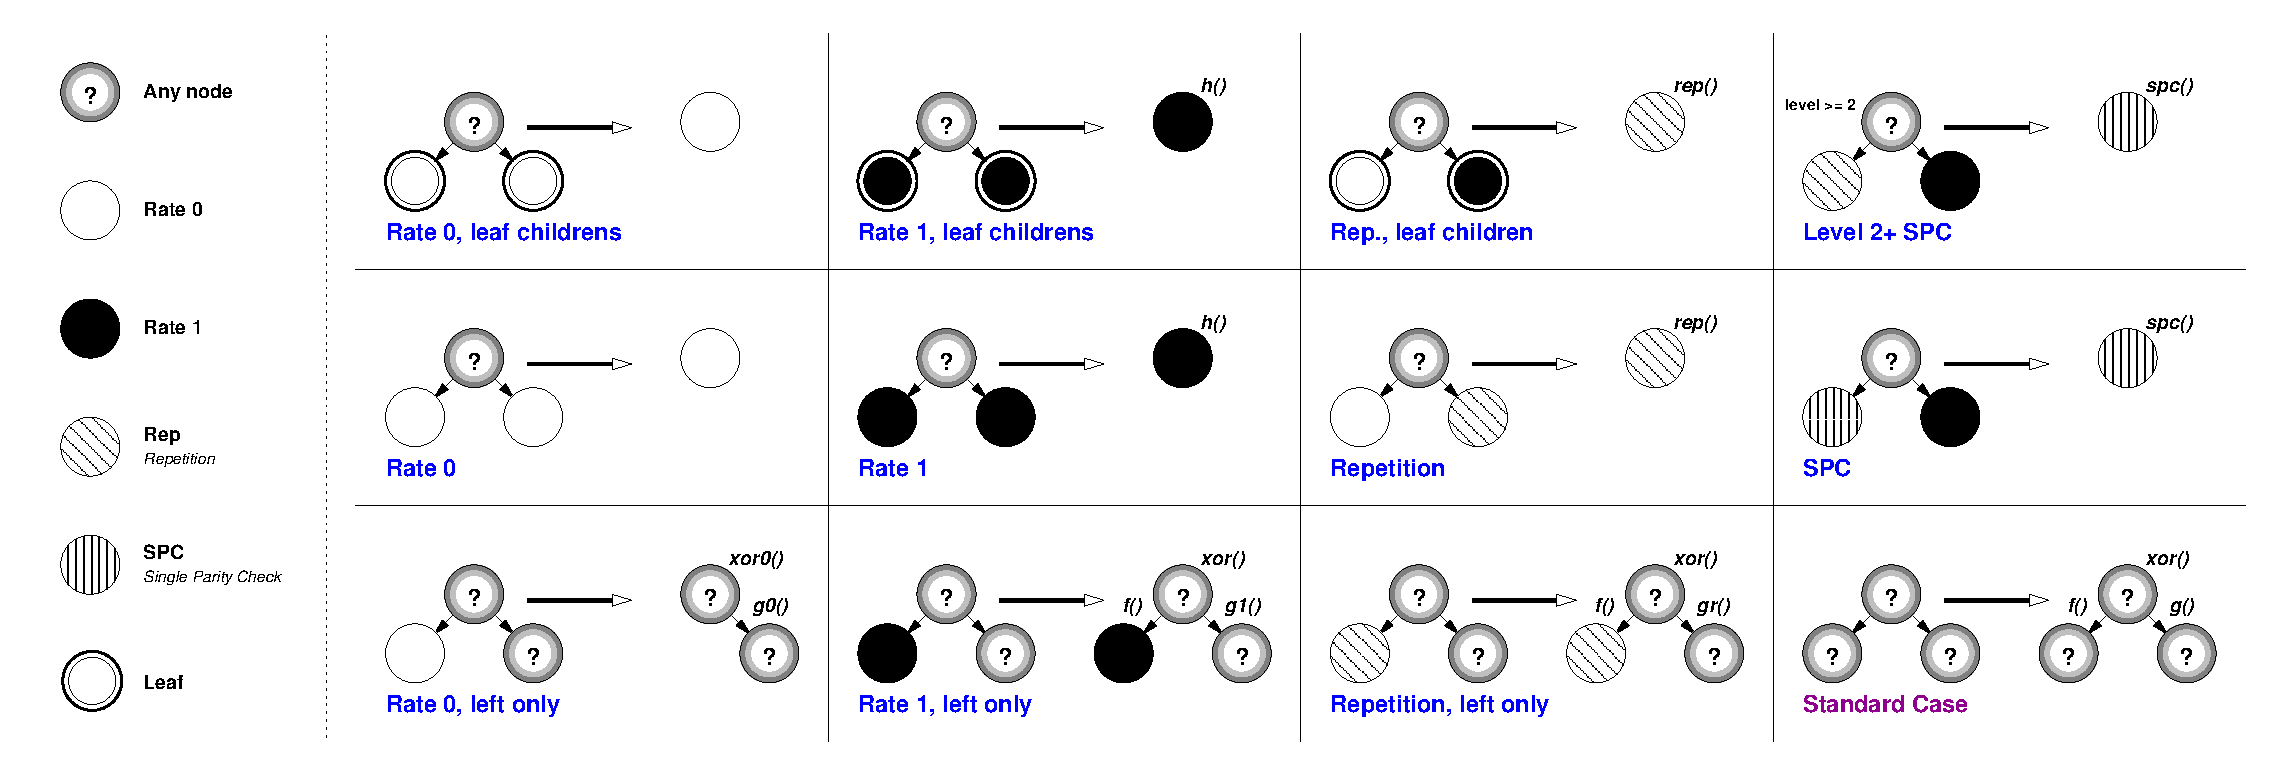
\includegraphics[width=1.0\textwidth]{polar/patterns}
%   \caption{Polar sub-tree rewriting rules for processing specialization.}
%   \label{fig:polar_patterns}
% \end{figure}

\begin{figure}[htp]
  \centering
  % \begin{scaletikzpicturetowidth}{0.70\linewidth}
  \begin{tikzpicture}
    \node[draw=gray,     circle, minimum height=0.6cm, text=black, fill=gray!40                                                                              , label={[black,align=center]above:\small{Any}}                       ] (any)  at ( 0.0, 0.0) {};
    \node[draw=black,    circle, minimum height=0.6cm, text=black                                                                                            , label={[black,align=center]above:\small{Frozen bit}\\\small{(leaf)}}] (frz)  at ( 2.0, 0.0) {};
    \node[draw=black,    circle, minimum height=0.6cm, text=black, fill=black                                                                                , label={[black,align=center]above:\small{Info. bit}\\\small{(leaf)}} ] (ufrz) at ( 4.0, 0.0) {};
    \node[draw=Paired-1, circle, minimum height=0.6cm, text=black, preaction={fill=Paired-1!40}, pattern=north west lines, pattern color=black!80!Paired-1!70, label={[black,align=center]above:\small{\texttt{R0}}}               ] (r0)   at ( 6.0, 0.0) {};
    \node[draw=Paired-3, circle, minimum height=0.6cm, text=black, preaction={fill=Paired-3!40}, pattern=north east lines, pattern color=black!80!Paired-3!70, label={[black,align=center]above:\small{\texttt{R1}}}               ] (r1)   at ( 8.0, 0.0) {};
    \node[draw=Paired-7, circle, minimum height=0.6cm, text=black, preaction={fill=Paired-7!40}, pattern=crosshatch dots,  pattern color=black!80!Paired-7!70, label={[black,align=center]above:\small{\texttt{REP}}}              ] (rep)  at (10.0, 0.0) {};
    \node[draw=Paired-5, circle, minimum height=0.6cm, text=black, preaction={fill=Paired-5!40}, pattern=horizontal lines, pattern color=black!80!Paired-5!70, label={[black,align=center]above:\small{\texttt{SPC}$_\texttt{4}$}} ] (spc4) at (12.0, 0.0) {};
    \node[draw=Paired-9, circle, minimum height=0.6cm, text=black, preaction={fill=Paired-9!40}, pattern=grid,             pattern color=black!80!Paired-9!70, label={[black,align=center]above:\small{\texttt{SPC}$_\texttt{4+}$}}] (spc)  at (14.0, 0.0) {};
  \end{tikzpicture}

  \begin{tikzpicture}
    \draw[black, dashed] (0,0.0) -- (16,0.0) node [midway, text=black] {};
  \end{tikzpicture}

  \begin{tikzpicture}%[scale=\tikzscale]
    \node[draw=black, circle, minimum height=0.6cm, text=black              ] (l1_g0) at (0.0, 0.0) {};
    \node[draw=black, circle, minimum height=0.6cm, text=black              ] (l1_g1) at (1.0, 0.0) {};
    \node[draw=gray,  circle, minimum height=0.6cm, text=black, fill=gray!40] (l0_g0) at (0.5, 1.0) {};

    \draw[->,>=latex] (l0_g0) -- (l1_g0) node [midway, above, text=black, yshift=-0.125cm, xshift=-0.075cm] {\tiny{$f$}};
    \draw[->,>=latex] (l0_g0) -- (l1_g1) node [midway, above, text=black, yshift=-0.125cm, xshift=+0.075cm] {\tiny{$g$}};
    \draw[->,>=latex] (l0_g0) to [out=0,in=60,looseness=4] (l0_g0) node [right, text=black, xshift=0.225cm, yshift=0.075cm] {\tiny{$xor$}};

    \draw[->,>=latex, black, line width=1.0pt] (1.2, 0.5) -> (1.8, 0.5);

    \node[draw=white, circle, minimum height=0.6cm] (l1_g0_fake) at (2.0, 0.0) {};
    \node[draw=white, circle, minimum height=0.6cm] (l1_g1_fake) at (3.0, 0.0) {};
    \node[draw=white, circle, minimum height=0.6cm] (l0_g0_fake) at (2.5, 1.0) {};

    \node[draw=Paired-1, circle, minimum height=0.6cm, text=black, preaction={fill=Paired-1!40}, pattern=north west lines, pattern color=black!80!Paired-1!70] (l0_g0_t) at (2.5, 0.5) {};
  \end{tikzpicture}
  \begin{tikzpicture}
    \draw (0,-0.3) -- (0,1.45) node [midway, text=black] {};
  \end{tikzpicture}
  \begin{tikzpicture}
    \node[draw=black, circle, minimum height=0.6cm, text=black, fill=black  ] (l1_g0) at (0.0, 0.0) {};
    \node[draw=black, circle, minimum height=0.6cm, text=black, fill=black  ] (l1_g1) at (1.0, 0.0) {};
    \node[draw=gray,  circle, minimum height=0.6cm, text=black, fill=gray!40] (l0_g0) at (0.5, 1.0) {};

    \draw[->,>=latex] (l0_g0) -- (l1_g0) node [midway, above, text=black, yshift=-0.125cm, xshift=-0.075cm] {\tiny{$f$}};
    \draw[->,>=latex] (l0_g0) -- (l1_g1) node [midway, above, text=black, yshift=-0.125cm, xshift=+0.075cm] {\tiny{$g$}};
    \draw[->,>=latex] (l0_g0) to [out=0,in=60,looseness=4] (l0_g0) node [right, text=black, xshift=0.225cm, yshift=0.075cm] {\tiny{$xor$}};

    \draw[->,>=latex, black, line width=1.0pt] (1.2, 0.5) -> (1.8, 0.5);

    \node[draw=white, circle, minimum height=0.6cm] (l1_g0_fake) at (2.0, 0.0) {};
    \node[draw=white, circle, minimum height=0.6cm] (l1_g1_fake) at (3.0, 0.0) {};
    \node[draw=white, circle, minimum height=0.6cm] (l0_g0_fake) at (2.5, 1.0) {};

    \node[draw=Paired-3, circle, minimum height=0.6cm, text=black, preaction={fill=Paired-3!40}, pattern=north east lines, pattern color=black!80!Paired-3!70] (l0_g0_t) at (2.5, 0.5) {};

    \draw[->,>=latex] (l0_g0_t) to [out=120,in=60,looseness=4] (l0_g0_t) node [left, text=black, yshift=0.45cm, xshift=0.1cm] {\tiny{$h$}};
  \end{tikzpicture}
  \begin{tikzpicture}
    \draw (0,-0.3) -- (0,1.45) node [midway, text=black] {};
  \end{tikzpicture}
  \begin{tikzpicture}
    \node[draw=black, circle, minimum height=0.6cm, text=black              ] (l1_g0) at (0.0, 0.0) {};
    \node[draw=black, circle, minimum height=0.6cm, text=black, fill=black  ] (l1_g1) at (1.0, 0.0) {};
    \node[draw=gray,  circle, minimum height=0.6cm, text=black, fill=gray!40] (l0_g0) at (0.5, 1.0) {};

    \draw[->,>=latex] (l0_g0) -- (l1_g0) node [midway, above, text=black, yshift=-0.125cm, xshift=-0.075cm] {\tiny{$f$}};
    \draw[->,>=latex] (l0_g0) -- (l1_g1) node [midway, above, text=black, yshift=-0.125cm, xshift=+0.075cm] {\tiny{$g$}};
    \draw[->,>=latex] (l0_g0) to [out=0,in=60,looseness=4] (l0_g0) node [right, text=black, xshift=0.225cm, yshift=0.075cm] {\tiny{$xor$}};

    \draw[->,>=latex, black, line width=1.0pt] (1.2, 0.5) -> (1.8, 0.5);

    \node[draw=white, circle, minimum height=0.6cm] (l1_g0_t_fake) at (2.0, 0.0) {};
    \node[draw=white, circle, minimum height=0.6cm] (l1_g1_t_fake) at (3.0, 0.0) {};
    \node[draw=white, circle, minimum height=0.6cm] (l0_g0_t_fake) at (2.5, 1.0) {};

    \node[draw=Paired-7, circle, minimum height=0.6cm, text=black, preaction={fill=Paired-7!40}, pattern=crosshatch dots,  pattern color=black!80!Paired-7!70] (l0_g0_t) at (2.5, 0.5) {};

    \draw[->,>=latex] (l0_g0_t) to [out=120,in=60,looseness=4] (l0_g0_t) node [left, text=black, yshift=0.45cm, xshift=0.2cm] {\tiny{$rep$}};
  \end{tikzpicture}
  \begin{tikzpicture}
    \draw (0,-0.3) -- (0,1.45) node [midway, text=black] {};
  \end{tikzpicture}
  \begin{tikzpicture}
    \node[draw=Paired-7, circle, minimum height=0.6cm, text=black, preaction={fill=Paired-7!40}, pattern=crosshatch dots,  pattern color=black!80!Paired-7!70] (l1_g0) at (0.0, 0.0) {};
    \node[draw=Paired-3, circle, minimum height=0.6cm, text=black, preaction={fill=Paired-3!40}, pattern=north east lines, pattern color=black!80!Paired-3!70] (l1_g1) at (1.0, 0.0) {};
    \node[draw=gray,     circle, minimum height=0.6cm, text=black, fill=gray!40                                                                              ] (l0_g0) at (0.5, 1.0) {};

    \draw[->,>=latex] (l0_g0) -- (l1_g0) node [midway, above, text=black, yshift=-0.125cm, xshift=-0.075cm] {\tiny{$f$}};
    \draw[->,>=latex] (l0_g0) -- (l1_g1) node [midway, above, text=black, yshift=-0.125cm, xshift=+0.075cm] {\tiny{$g$}};
    \draw[->,>=latex] (l0_g0) to [out=0,in=60,looseness=4] (l0_g0) node [right, text=black, xshift=0.225cm, yshift=0.075cm] {\tiny{$xor$}};

    \draw[->,>=latex, black, line width=1.0pt] (1.2, 0.5) -> (1.8, 0.5);

    \node[draw=white, circle, minimum height=0.6cm] (l1_g0_t_fake) at (2.0, 0.0) {};
    \node[draw=white, circle, minimum height=0.6cm] (l1_g1_t_fake) at (3.0, 0.0) {};
    \node[draw=white, circle, minimum height=0.6cm] (l0_g0_t_fake) at (2.5, 1.0) {};

    \node[draw=Paired-5, circle, minimum height=0.6cm, text=black, preaction={fill=Paired-5!40}, pattern=horizontal lines, pattern color=black!80!Paired-5!70] (l0_g0_t) at (2.5, 0.5) {};

    \draw[->,>=latex] (l0_g0_t) to [out=120,in=60,looseness=4] (l0_g0_t) node [left, text=black, yshift=0.45cm, xshift=0.2cm] {\tiny{$spc$}};
  \end{tikzpicture}

  \begin{tikzpicture}
    \draw[black] (0,0.0) -- (16,0.0) node [midway, text=black] {};
  \end{tikzpicture}

  \begin{tikzpicture}%[scale=\tikzscale]
    \node[draw=Paired-1, circle, minimum height=0.6cm, text=black, preaction={fill=Paired-1!40}, pattern=north west lines, pattern color=black!80!Paired-1!70] (l1_g0) at (0.0, 0.0) {};
    \node[draw=Paired-1, circle, minimum height=0.6cm, text=black, preaction={fill=Paired-1!40}, pattern=north west lines, pattern color=black!80!Paired-1!70] (l1_g1) at (1.0, 0.0) {};
    \node[draw=gray,     circle, minimum height=0.6cm, text=black, fill=gray!40                                                                              ] (l0_g0) at (0.5, 1.0) {};

    \draw[->,>=latex] (l0_g0) -- (l1_g0) node [midway, above, text=black, yshift=-0.125cm, xshift=-0.075cm] {\tiny{$f$}};
    \draw[->,>=latex] (l0_g0) -- (l1_g1) node [midway, above, text=black, yshift=-0.125cm, xshift=+0.075cm] {\tiny{$g$}};
    \draw[->,>=latex] (l0_g0) to [out=0,in=60,looseness=4] (l0_g0) node [right, text=black, xshift=0.225cm, yshift=0.075cm] {\tiny{$xor$}};

    \draw[->,>=latex, black, line width=1.0pt] (1.2, 0.5) -> (1.8, 0.5);

    \node[draw=white, circle, minimum height=0.6cm] (l1_g0_t_fake) at (2.0, 0.0) {};
    \node[draw=white, circle, minimum height=0.6cm] (l1_g1_t_fake) at (3.0, 0.0) {};
    \node[draw=white, circle, minimum height=0.6cm] (l0_g0_t_fake) at (2.5, 1.0) {};

    \node[draw=Paired-1, circle, minimum height=0.6cm, text=black, preaction={fill=Paired-1!40}, pattern=north west lines, pattern color=black!80!Paired-1!70] (l0_g0_t) at (2.5, 0.5) {};
  \end{tikzpicture}
  \begin{tikzpicture}
    \draw (0,-0.3) -- (0,1.45) node [midway, text=black] {};
  \end{tikzpicture}
  \begin{tikzpicture}
    \node[draw=Paired-3, circle, minimum height=0.6cm, text=black, preaction={fill=Paired-3!40}, pattern=north east lines, pattern color=black!80!Paired-3!70] (l1_g0) at (0.0, 0.0) {};
    \node[draw=Paired-3, circle, minimum height=0.6cm, text=black, preaction={fill=Paired-3!40}, pattern=north east lines, pattern color=black!80!Paired-3!70] (l1_g1) at (1.0, 0.0) {};
    \node[draw=gray,     circle, minimum height=0.6cm, text=black, fill=gray!40                                                                              ] (l0_g0) at (0.5, 1.0) {};

    \draw[->,>=latex] (l0_g0) -- (l1_g0) node [midway, above, text=black, yshift=-0.125cm, xshift=-0.075cm] {\tiny{$f$}};
    \draw[->,>=latex] (l0_g0) -- (l1_g1) node [midway, above, text=black, yshift=-0.125cm, xshift=+0.075cm] {\tiny{$g$}};
    \draw[->,>=latex] (l0_g0) to [out=0,in=60,looseness=4] (l0_g0) node [right, text=black, xshift=0.225cm, yshift=0.075cm] {\tiny{$xor$}};

    \draw[->,>=latex, black, line width=1.0pt] (1.2, 0.5) -> (1.8, 0.5);

    \node[draw=white, circle, minimum height=0.6cm] (l1_g0_t_fake) at (2.0, 0.0) {};
    \node[draw=white, circle, minimum height=0.6cm] (l1_g1_t_fake) at (3.0, 0.0) {};
    \node[draw=white, circle, minimum height=0.6cm] (l0_g0_t_fake) at (2.5, 1.0) {};

    \node[draw=Paired-3, circle, minimum height=0.6cm, text=black, preaction={fill=Paired-3!40}, pattern=north east lines, pattern color=black!80!Paired-3!70] (l0_g0_t) at (2.5, 0.5) {};

    \draw[->,>=latex] (l0_g0_t) to [out=120,in=60,looseness=4] (l0_g0_t) node [left, text=black, yshift=0.45cm, xshift=0.1cm] {\tiny{$h$}};
  \end{tikzpicture}
  \begin{tikzpicture}
    \draw (0,-0.3) -- (0,1.45) node [midway, text=black] {};
  \end{tikzpicture}
  \begin{tikzpicture}
    \node[draw=Paired-1, circle, minimum height=0.6cm, text=black, preaction={fill=Paired-1!40}, pattern=north west lines, pattern color=black!80!Paired-1!70] (l1_g0) at (0.0, 0.0) {};
    \node[draw=Paired-7, circle, minimum height=0.6cm, text=black, preaction={fill=Paired-7!40}, pattern=crosshatch dots,  pattern color=black!80!Paired-7!70] (l1_g1) at (1.0, 0.0) {};
    \node[draw=gray,     circle, minimum height=0.6cm, text=black, fill=gray!40                                                                              ] (l0_g0) at (0.5, 1.0) {};

    \draw[->,>=latex] (l0_g0) -- (l1_g0) node [midway, above, text=black, yshift=-0.125cm, xshift=-0.075cm] {\tiny{$f$}};
    \draw[->,>=latex] (l0_g0) -- (l1_g1) node [midway, above, text=black, yshift=-0.125cm, xshift=+0.075cm] {\tiny{$g$}};
    \draw[->,>=latex] (l0_g0) to [out=0,in=60,looseness=4] (l0_g0) node [right, text=black, xshift=0.225cm, yshift=0.075cm] {\tiny{$xor$}};

    \draw[->,>=latex, black, line width=1.0pt] (1.2, 0.5) -> (1.8, 0.5);

    \node[draw=white, circle, minimum height=0.6cm] (l1_g0_t_fake) at (2.0, 0.0) {};
    \node[draw=white, circle, minimum height=0.6cm] (l1_g1_t_fake) at (3.0, 0.0) {};
    \node[draw=white, circle, minimum height=0.6cm] (l0_g0_t_fake) at (2.5, 1.0) {};

    \node[draw=Paired-7, circle, minimum height=0.6cm, text=black, preaction={fill=Paired-7!40}, pattern=crosshatch dots,  pattern color=black!80!Paired-7!70] (l0_g0_t) at (2.5, 0.5) {};

    \draw[->,>=latex] (l0_g0_t) to [out=120,in=60,looseness=4] (l0_g0_t) node [left, text=black, yshift=0.45cm, xshift=0.2cm] {\tiny{$rep$}};
  \end{tikzpicture}
  \begin{tikzpicture}
    \draw (0,-0.3) -- (0,1.45) node [midway, text=black] {};
  \end{tikzpicture}
  \begin{tikzpicture}
    \node[draw=Paired-5, circle, minimum height=0.6cm, text=black, preaction={fill=Paired-5!40}, pattern=horizontal lines, pattern color=black!80!Paired-5!70] (l1_g0) at (0.0, 0.0) {};
    \node[draw=Paired-3, circle, minimum height=0.6cm, text=black, preaction={fill=Paired-3!40}, pattern=north east lines, pattern color=black!80!Paired-3!70] (l1_g1) at (1.0, 0.0) {};
    \node[draw=gray,     circle, minimum height=0.6cm, text=black, fill=gray!40                                                                              ] (l0_g0) at (0.5, 1.0) {};

    \draw[->,>=latex] (l0_g0) -- (l1_g0) node [midway, above, text=black, yshift=-0.125cm, xshift=-0.075cm] {\tiny{$f$}};
    \draw[->,>=latex] (l0_g0) -- (l1_g1) node [midway, above, text=black, yshift=-0.125cm, xshift=+0.075cm] {\tiny{$g$}};
    \draw[->,>=latex] (l0_g0) to [out=0,in=60,looseness=4] (l0_g0) node [right, text=black, xshift=0.225cm, yshift=0.075cm] {\tiny{$xor$}};

    \draw[->,>=latex, black, line width=1.0pt] (1.2, 0.5) -> (1.8, 0.5);

    \node[draw=white, circle, minimum height=0.6cm] (l1_g0_t_fake) at (2.0, 0.0) {};
    \node[draw=white, circle, minimum height=0.6cm] (l1_g1_t_fake) at (3.0, 0.0) {};
    \node[draw=white, circle, minimum height=0.6cm] (l0_g0_t_fake) at (2.5, 1.0) {};

    \node[draw=Paired-9, circle, minimum height=0.6cm, text=black, preaction={fill=Paired-9!40}, pattern=grid, pattern color=black!80!Paired-9!70] (l0_g0_t) at (2.5, 0.5) {};

    \draw[->,>=latex] (l0_g0_t) to [out=120,in=60,looseness=4] (l0_g0_t) node [left, text=black, yshift=0.45cm, xshift=0.2cm] {\tiny{$spc$}};
  \end{tikzpicture}

  \begin{tikzpicture}
    \draw[black] (0,0.0) -- (16,0.0) node [midway, text=black] {};
  \end{tikzpicture}

  \begin{tikzpicture}%[scale=\tikzscale]
    \node[draw=Paired-1, circle, minimum height=0.6cm, text=black, preaction={fill=Paired-1!40}, pattern=north west lines, pattern color=black!80!Paired-1!70] (l1_g0) at (0.0, 0.0) {};
    \node[draw=gray,     circle, minimum height=0.6cm, text=black, fill=gray!40                                       ] (l1_g1) at (1.0, 0.0) {};
    \node[draw=gray,     circle, minimum height=0.6cm, text=black, fill=gray!40                                       ] (l0_g0) at (0.5, 1.0) {};

    \draw[->,>=latex] (l0_g0) -- (l1_g0) node [midway, above, text=black, yshift=-0.125cm, xshift=-0.075cm] {\tiny{$f$}};
    \draw[->,>=latex] (l0_g0) -- (l1_g1) node [midway, above, text=black, yshift=-0.125cm, xshift=+0.075cm] {\tiny{$g$}};
    \draw[->,>=latex] (l0_g0) to [out=0,in=60,looseness=4] (l0_g0) node [right, text=black, xshift=0.225cm, yshift=0.075cm] {\tiny{$xor$}};

    \draw[->,>=latex, black, line width=1.0pt] (1.2, 0.5) -> (1.8, 0.5);

    \node[draw=gray,  circle, minimum height=0.6cm, text=black, fill=gray!40] (l1_g1_t) at (3.0, 0.0) {};
    \node[draw=gray,  circle, minimum height=0.6cm, text=black, fill=gray!40] (l0_g0_t) at (2.5, 1.0) {};

    \draw[->,>=latex] (l0_g0_t) -- (l1_g1_t) node [midway, above, text=black, yshift=-0.125cm, xshift=+0.15cm] {\tiny{$g_0$}};
    \draw[->,>=latex] (l0_g0_t) to [out=180,in=120,looseness=4] (l0_g0_t) node [right, text=black, xshift=-0.9cm, yshift=0.075cm] {\tiny{$xor$}};
  \end{tikzpicture}
  \begin{tikzpicture}
    \draw (0,-0.3) -- (0,1.45) node [midway, text=black] {};
  \end{tikzpicture}
  \begin{tikzpicture}
    \node[draw=Paired-3, circle, minimum height=0.6cm, text=black, preaction={fill=Paired-3!40}, pattern=north east lines, pattern color=black!80!Paired-3!70] (l1_g0) at (0.0, 0.0) {};
    \node[draw=gray,     circle, minimum height=0.6cm, text=black, fill=gray!40                                                                              ] (l1_g1) at (1.0, 0.0) {};
    \node[draw=gray,     circle, minimum height=0.6cm, text=black, fill=gray!40                                                                              ] (l0_g0) at (0.5, 1.0) {};

    \draw[->,>=latex] (l0_g0) -- (l1_g0) node [midway, above, text=black, yshift=-0.125cm, xshift=-0.075cm] {\tiny{$f$}};
    \draw[->,>=latex] (l0_g0) -- (l1_g1) node [midway, above, text=black, yshift=-0.125cm, xshift=+0.075cm] {\tiny{$g$}};
    \draw[->,>=latex] (l0_g0) to [out=0,in=60,looseness=4] (l0_g0) node [right, text=black, xshift=0.225cm, yshift=0.075cm] {\tiny{$xor$}};

    \draw[->,>=latex, black, line width=1.0pt] (1.2, 0.5) -> (1.8, 0.5);

    \node[draw=Paired-3, circle, minimum height=0.6cm, text=black, preaction={fill=Paired-3!40}, pattern=north east lines, pattern color=black!80!Paired-3!70] (l1_g0_t) at (2.0, 0.0) {};
    \node[draw=gray,     circle, minimum height=0.6cm, text=black, fill=gray!40                                                                              ] (l1_g1_t) at (3.0, 0.0) {};
    \node[draw=gray,     circle, minimum height=0.6cm, text=black, fill=gray!40                                                                              ] (l0_g0_t) at (2.5, 1.0) {};

    \draw[->,>=latex] (l0_g0_t) -- (l1_g0_t) node [midway, above, text=black, yshift=-0.125cm, xshift=-0.075cm] {\tiny{$f$}};
    \draw[->,>=latex] (l0_g0_t) -- (l1_g1_t) node [midway, above, text=black, yshift=-0.125cm, xshift=+0.150cm] {\tiny{$g_1$}};
    \draw[->,>=latex] (l0_g0_t) to [out=180,in=120,looseness=4] (l0_g0_t) node [right, text=black, xshift=-0.9cm, yshift=0.075cm] {\tiny{$xor$}};
  \end{tikzpicture}
  \begin{tikzpicture}
    \draw (0,-0.3) -- (0,1.45) node [midway, text=black] {};
  \end{tikzpicture}
  \begin{tikzpicture}
    \node[draw=Paired-7, circle, minimum height=0.6cm, text=black, preaction={fill=Paired-7!40}, pattern=crosshatch dots,  pattern color=black!80!Paired-7!70] (l1_g0) at (0.0, 0.0) {};
    \node[draw=gray,     circle, minimum height=0.6cm, text=black, fill=gray!40                                                                              ] (l1_g1) at (1.0, 0.0) {};
    \node[draw=gray,     circle, minimum height=0.6cm, text=black, fill=gray!40                                                                              ] (l0_g0) at (0.5, 1.0) {};

    \draw[->,>=latex] (l0_g0) -- (l1_g0) node [midway, above, text=black, yshift=-0.125cm, xshift=-0.075cm] {\tiny{$f$}};
    \draw[->,>=latex] (l0_g0) -- (l1_g1) node [midway, above, text=black, yshift=-0.125cm, xshift=+0.075cm] {\tiny{$g$}};
    \draw[->,>=latex] (l0_g0) to [out=0,in=60,looseness=4] (l0_g0) node [right, text=black, xshift=0.225cm, yshift=0.075cm] {\tiny{$xor$}};

    \draw[->,>=latex, black, line width=1.0pt] (1.2, 0.5) -> (1.8, 0.5);

    \node[draw=Paired-7, circle, minimum height=0.6cm, text=black, preaction={fill=Paired-7!40}, pattern=crosshatch dots,  pattern color=black!80!Paired-7!70] (l1_g0_t) at (2.0, 0.0) {};
    \node[draw=gray,     circle, minimum height=0.6cm, text=black, fill=gray!40                                                                              ] (l1_g1_t) at (3.0, 0.0) {};
    \node[draw=gray,     circle, minimum height=0.6cm, text=black, fill=gray!40                                                                              ] (l0_g0_t) at (2.5, 1.0) {};

    \draw[->,>=latex] (l0_g0_t) -- (l1_g0_t) node [midway, above, text=black, yshift=-0.125cm, xshift=-0.075cm] {\tiny{$f$}};
    \draw[->,>=latex] (l0_g0_t) -- (l1_g1_t) node [midway, above, text=black, yshift=-0.125cm, xshift=+0.150cm] {\tiny{$g_r$}};
    \draw[->,>=latex] (l0_g0_t) to [out=180,in=120,looseness=4] (l0_g0_t) node [right, text=black, xshift=-0.9cm, yshift=0.075cm] {\tiny{$xor$}};
  \end{tikzpicture}
  \begin{tikzpicture}
    \draw (0,-0.3) -- (0,1.45) node [midway, text=black] {};
  \end{tikzpicture}
  \begin{tikzpicture}
    \node[draw=Paired-9, circle, minimum height=0.6cm, text=black, preaction={fill=Paired-9!40}, pattern=grid,             pattern color=black!80!Paired-9!70] (l1_g0) at (0.0, 0.0) {};
    \node[draw=Paired-3, circle, minimum height=0.6cm, text=black, preaction={fill=Paired-3!40}, pattern=north east lines, pattern color=black!80!Paired-3!70] (l1_g1) at (1.0, 0.0) {};
    \node[draw=gray,     circle, minimum height=0.6cm, text=black, fill=gray!40                                                                              ] (l0_g0) at (0.5, 1.0) {};

    \draw[->,>=latex] (l0_g0) -- (l1_g0) node [midway, above, text=black, yshift=-0.125cm, xshift=-0.075cm] {\tiny{$f$}};
    \draw[->,>=latex] (l0_g0) -- (l1_g1) node [midway, above, text=black, yshift=-0.125cm, xshift=+0.075cm] {\tiny{$g$}};
    \draw[->,>=latex] (l0_g0) to [out=0,in=60,looseness=4] (l0_g0) node [right, text=black, xshift=0.225cm, yshift=0.075cm] {\tiny{$xor$}};

    \draw[->,>=latex, black, line width=1.0pt] (1.2, 0.5) -> (1.8, 0.5);

    \node[draw=white, circle, minimum height=0.6cm] (l1_g0_fake) at (2.0, 0.0) {};
    \node[draw=white, circle, minimum height=0.6cm] (l1_g1_fake) at (3.0, 0.0) {};
    \node[draw=white, circle, minimum height=0.6cm] (l0_g0_fake) at (2.5, 1.0) {};

    \node[draw=Paired-9, circle, minimum height=0.6cm, text=black, preaction={fill=Paired-9!40}, pattern=grid, pattern color=black!80!Paired-9!70] (l0_g0_t) at (2.5, 0.5) {};

    \draw[->,>=latex] (l0_g0_t) to [out=120,in=60,looseness=4] (l0_g0_t) node [left, text=black, yshift=0.45cm, xshift=0.2cm] {\tiny{$spc$}};
  \end{tikzpicture}

  \caption{Polar sub-tree rewriting rules for processing specialization.}
  \label{fig:polar_patterns}
\end{figure}

For some sub-tree pattern configurations, the processing to be performed at the
root of such sub-trees can be simplified, or even skipped completely, for
instance when a node only has two frozen bit leaf children. To exploit such
properties, the decoder generator repeatedly applies the set of sub-tree
rewriting rules listed in Fig.~\ref{fig:polar_patterns} using a depth first
traversal to alter the node tags, until no rewriting rule applies anymore.

Each rewriting rule defines a subtree pattern \emph{selector}, a new \emph{tag}
for the subtree root, and the $f$, $g$, and $h$ \emph{processing functions} to
be applied, simplified or skipped for this node in the resulting decoder. A
\emph{null} $f$ (resp. $g$) function cuts the left (resp. right) child of the
node. From an implementation point of view, a rule is defined as a class, with a
\verb|match| function, and a set of functions $f$, $g$, and $h$. The current
set of rewriting rules can thus easily be enriched with new rules to generate
even more specialized versions.

Patterns on the first two rows result in cutting away both children. For
instance, the first rule, named \emph{Rate~0, leaf children}, cuts the two
frozen bit leaf children of the parent node, and tag it as \emph{Rate~0} (white
node). Processing is completely skipped on this node since the values of the
bits are unconditionally known. The \emph{Repetition} rules match subtrees where
only the rightmost leaf is black (tag \emph{Rate~1}), the others being frozen
bits. In this case, the whole subtree is cut and replaced by a more simple
processing. Moreover a single, specialized $rep$ function is applied on the node
instead of the three functions $f$, $g$ and $h$. The third line describes
partial cuts and specialization. For instance, the rule ``Repetition, left
only'' specializes the $g$ and $h$ functions to use, but does not prune the
recursive children processing.

Rewriting rules are ordered by priority (left to right, then top row to bottom
row in Fig.~\ref{fig:polar_patterns}), thus if more than one rule match an
encountered subtree, the highest priority rule is applied. The priority order is
chosen such as to favor strongest computation reducing rules over rules with
minor impact, and to ensure confluence by selecting the most specific pattern
first. Rules selectors can match on node tags and/or node levels (leaf, specific
level, above or below some level). A given rule is applied at most once on a
given node.

\begin{listing}[htp]
  \inputminted[frame=lines,linenos]{C++}{main/chapter3/src/polar/generated_sc_decoder.cpp}
  \caption{The final code generated corresponding to the pruned tree in
    Fig.~\ref{fig:tree_pruning_example}.}
  \label{lst:polar_patterns_example}
\end{listing}

Finally, once the tree has been fully specialized, the generator perform a
second tree traversal pass to output the resulting decoder. An example of such a
tree specialization process together with the generator output is shown in
Fig.~\ref{fig:tree_pruning_example} and in
Listing~\ref{lst:polar_patterns_example}. One may notice that in the
Listing~\ref{lst:polar_patterns_example} the polar API presented in
Listing~\ref{lst:polar_f_g_h_simd} is not compatible. This is because the polar
API has been previously simplified, in the real implementation the $f$, $g$ and
$h$ function implementation can be applied to a generic number of elements. In
Listing~\ref{lst:polar_patterns_example}, each operation (\verb|f|, \verb|rep|,
\verb|gr|, \verb|spc| and \verb|xo|) is applied on $4$ elements.

\paragraph{Source Code Compression}

\begin{figure}[htp]
  \centering
  \subfloat[][Without compression.]{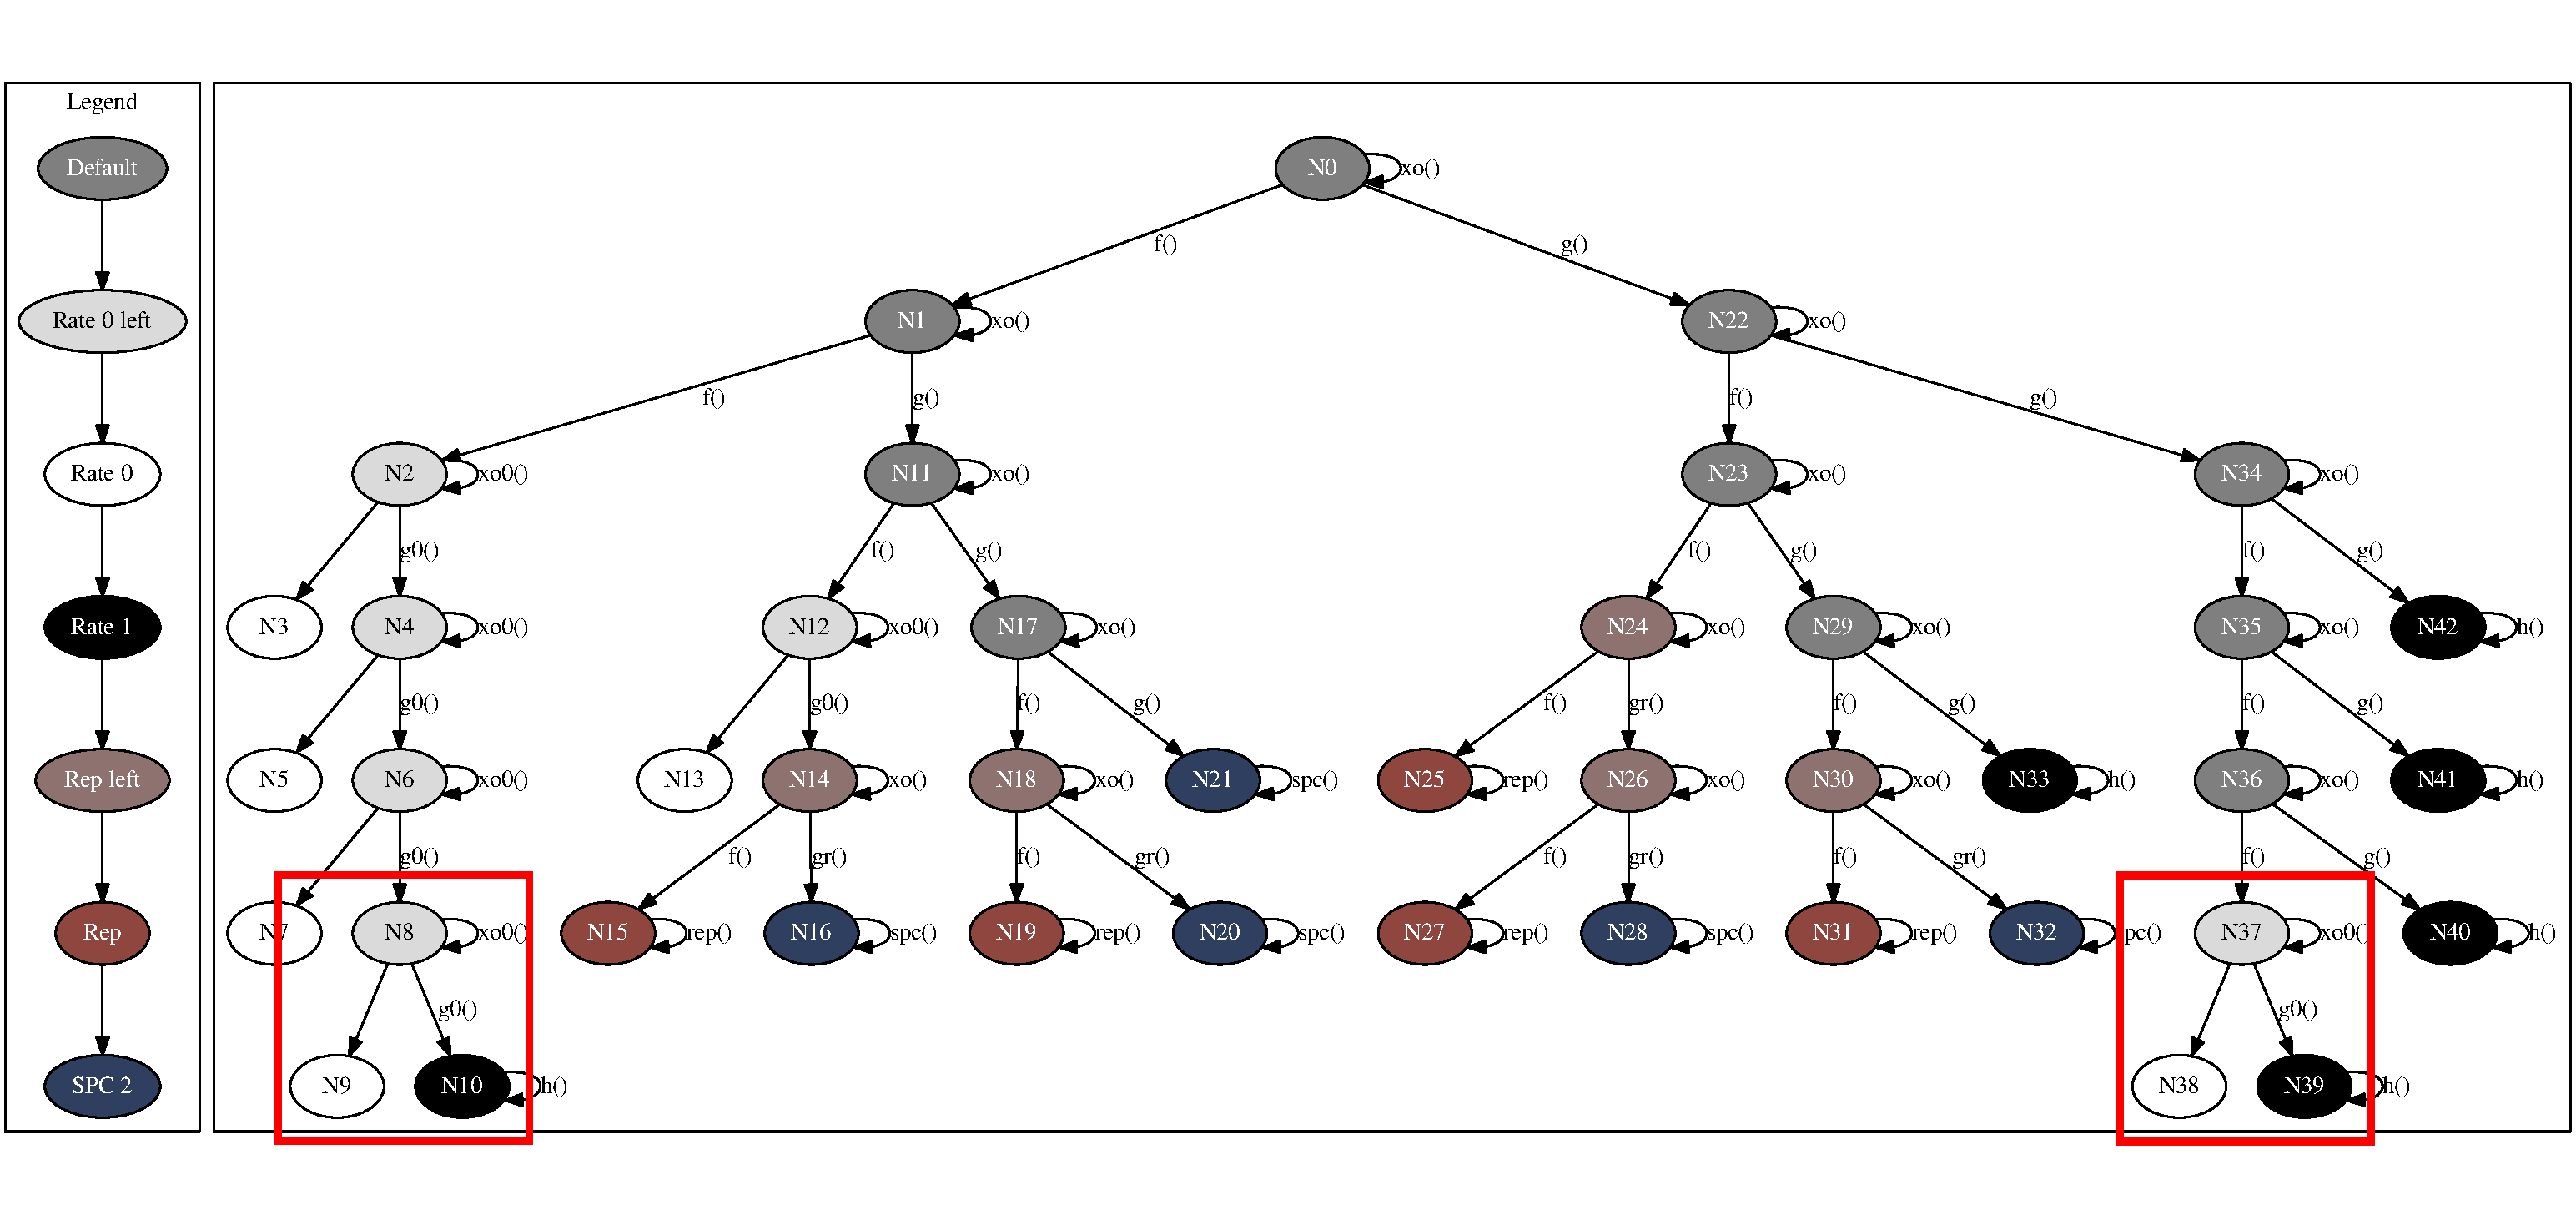
\includegraphics[height=7.5cm]{polar/sc_gen_compression/sc_gen_no_compression}\label{fig:eval_polar_sc_gen_compression_wo}}
  % \qquad
  \\
  \subfloat[][With compression.]{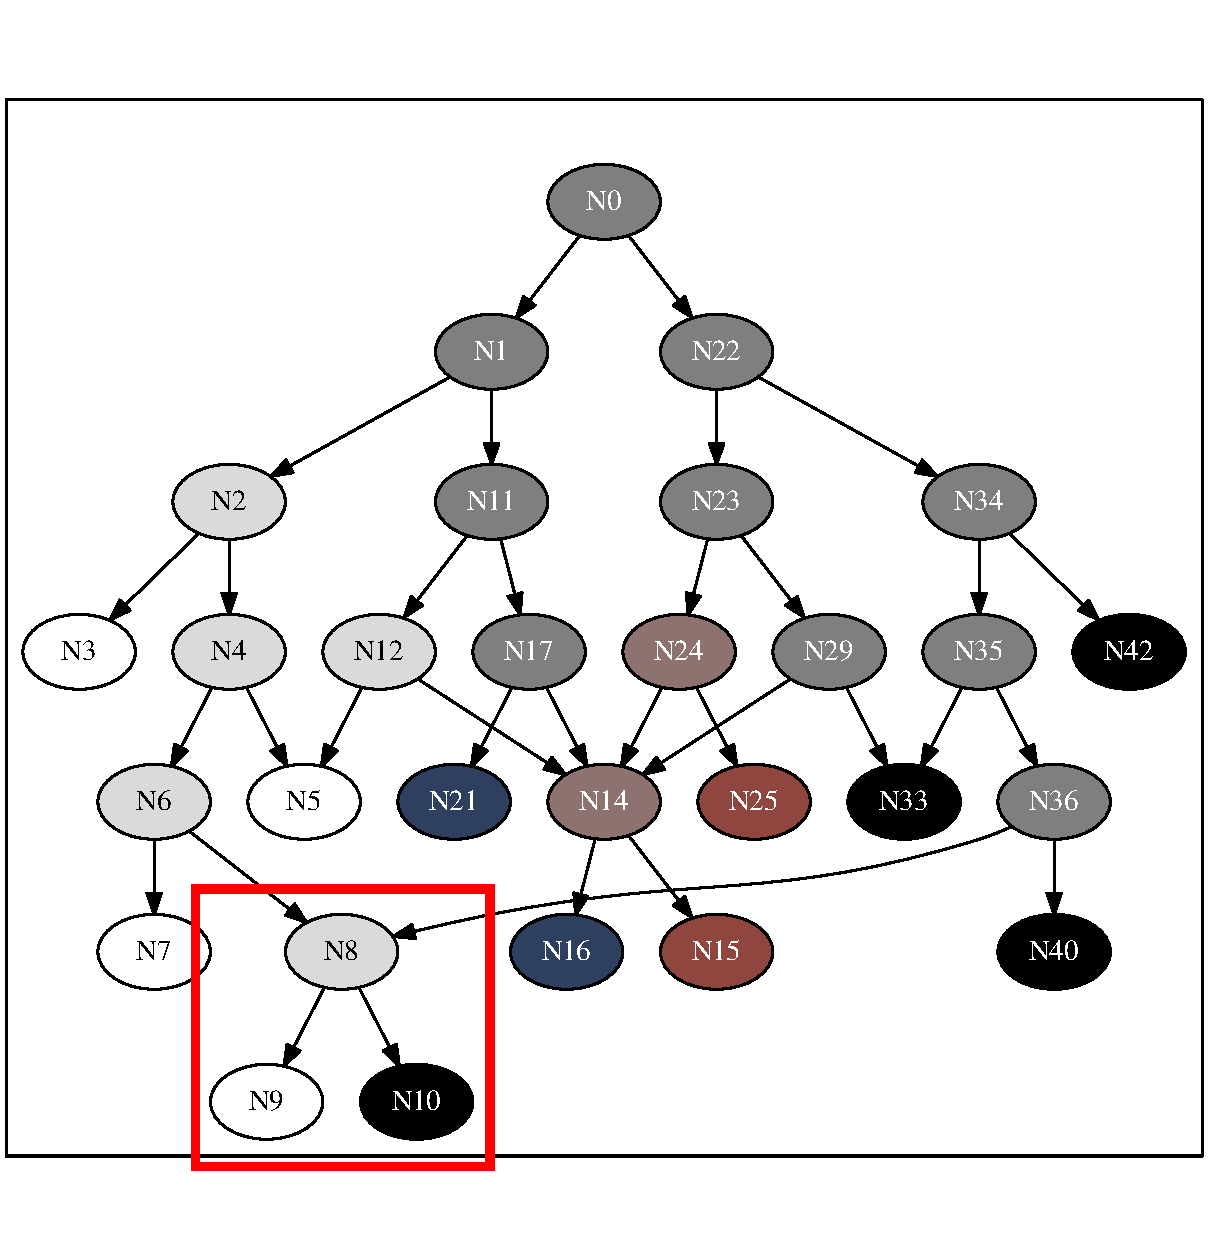
\includegraphics[height=7.5cm]{polar/sc_gen_compression/sc_gen_compression}\label{fig:eval_polar_sc_gen_compression_w}}
  \caption
    [Full polar decoding tree representation without and with compression.]
    {Full polar decoding tree representation ($N = 128, K = 64$) without and
    with the compression sub-tree folding algorithm.}
  \label{fig:eval_polar_sc_gen_compression}
\end{figure}

Decoders are generated as straight-line code (no recursive calls), with all node
computations put in sequence. This improves performance for small to medium
codeword size, up to the point where the compiled binary exceeds the L1I cache
size (this is also reported in~\cite{Giard2016b}). We mitigated this issue by
reducing decoder binary sizes using two compression techniques: 1) in the
generated code, we moved the buffer offsets from template arguments to function
arguments, which enabled the compiler to factorize more function calls than
before (improvement by a factor of 10), 2) we implemented a sub-tree folding
algorithm in the generator (see Fig.~\ref{fig:eval_polar_sc_gen_compression}),
to detect multiple occurrences of a same sub-tree and to put the corresponding
code into a dedicated function (improvement by a factor of 5 for $N=2^{16}$, the
compression ratio increases with the size of the tree).

\subsubsection{Dynamic Implementation}

\begin{itemize}
  \item \xmark~expliquer l'unrolling partiel à base de templates.
  \item \xmark~"dynamic" = "generic" présenté dans les algos
\end{itemize}

We extend the \AFFECT software with a new version of the Fast-SSC decoder,
called \emph{dynamic} decoder. This version uses the same building blocks (the
polar API) as the generated versions, but the same code is able to accommodate
with different frozen bit layouts and different parameters (length, SNR).
\Cxy{11} template specialization features are used to enable the compiler to
perform loop unrolling starting from a selected level in the decoding tree. It
is the first non-generated version (to the best of our knowledge) to support
both multi-precision (32-bit, 16-bit and 8-bit) and multi-SIMD strategies
(intra-frame or inter-frame).

% ceci est redit dans la section evaluation -----------------------------------
By design, generated decoders are still faster than the dynamic decoder (up to
20\%). However each generated decoder is optimized for a single SNR. For very
large frame sizes, the dynamic decoder outperforms generated decoders because
the heavily unrolled generated decoders exceed Level 1 instruction cache sizeF
capacity.
% ceci est redit dans la section evaluation -----------------------------------

\subsubsection{LLRs and Partial Sum Memory Management}

The decoder stores its state using two data buffers, one for the LLR values
($\lambda$) and the other for the bits (partial sums $s$). The ``logical'' tree
layout is implemented as a simple and efficient \emph{heap} vector data layout.
Traversing the tree therefore corresponds to moving through the array, at
different offsets and considering different index intervals. The LLR offset is
computed from the graph depth~$d$ (or the node vertical indexing) as follows:
%\begin{equation}
%  off_{\lambda}(d) = \begin{cases}
%    0                                         &\text{$d = 0$},\\
%    \sum\limits_{i = 1}^{d} \frac{N}{2^{i-1}} &\text{otherwise.}
%\end{cases}
%\end{equation}
\begin{equation}
  off_{\lambda}(d = 0) = 0,~off_{\lambda}(d > 0) =
  \sum\limits_{i = 1}^{d} \frac{N}{2^{i-1}}.
\end{equation}
Given~$l$ the lane (or the node horizontal indexing), the bit offset is
determined as follows:
\begin{equation}
  off_{s}(d,l) = \frac{N}{2^d} \times l.
\end{equation}
The LLR buffer size is $2N$ and the bit buffer is $N$, for a frame of $N$ bits.
Thus, the memory footprint per frame is:
\begin{equation}
  mem_{fp} = N \times (2 \times \sizeof(LLR) + \sizeof(bit)).
\end{equation}
LLRs element size is 4 bytes (float) or 1 byte (fixed point numbers). The
inter-SIMD version also employs a \emph{bit packing} memory footprint reduction
technique~\cite{LeGal2015a} to pack several bits together by using shifts and
masking instructions.

\subsection{Successive Cancellation List Decoders}

\subsubsection{Software implementation optimizations}
\label{sec:polar_implem}

The genericity and flexibility of the formerly described decoder prevent from
using some optimizations. Unrolling the description as in~\cite{Sarkis2016} is
not possible at runtime, although code generation could be used to produce an
unrolled version of any decoder as in \cite{Cassagne2015c}. Moreover, in the
case of large code lengths, the unrolling strategy can generate very large
compiled binary files. This can cause instruction cache misses that would
dramatically impact the decoder throughput. On the contrary, the size of the
executable files of the proposed decoder are constant with respect to the code
parameters ($N$, $K$, $L$). The number of cycles lost due to cache misses is,
according to our experiments, less than 0.01\% of the total number of cycles.
Still, some implementation improvements are necessary in order to be competitive
with specific unrolled decoders of the literature. The software library for
polar codes from \cite{Cassagne2015c,Cassagne2016b} enables to benefit from
the SIMD instructions for various target architectures. Optimizations of CRC
checking benefit to both the non-adaptive and adaptive versions of the CA-SCL
algorithms. The new sorting technique presented in
Section~\ref{sec:polar_sorting} can be applied to each variation of the SCL
algorithm. Finally, an efficient implementation of the partial sums memory
management is proposed. It is particularly effective for short polar codes.

\subsubsection{Improving Cyclic Redundancy Checking}
\label{sec:polar_crc}

By profiling the Adaptive SCL decoder, one may observe that a significant amount
of time is spent to process the cyclic redundancy checks. Its computational
complexity is O($LN$) versus the computational complexity of the SCL decoding,
O($LN\log N$). The first is not negligible compared to the second.

In the adaptive decoder, the CRC verification is performed a first time after
the SC decoding. In the following, we show how to reduce the computational
complexity of these CRC verifications.

First, an efficient CRC checking code has been implemented. Whenever the decoder
needs to check the CRC, the bits are packed and then computed 32 by 32. In order
to further speed up the implementation, a lookup table used to store
pre-computed CRC sub-sequences, and thus reduce the computational complexity.
The size of the lookup table is 1 KB.

After a regular SC decoding, a decision vector of size $N$ is produced. Then,
the $K$ information bits must be extracted to apply cyclic redundancy check. The
profiling of our decoder description shows that this extraction takes a
significant amount of time compared to the check operation itself. Consequently,
a specific extraction function was implemented. This function takes advantage of
the leaf node type knowledge to perform efficient multi-element copies.

Concerning SCL decoding, it is possible to sort the candidates according to
their respective metrics and then to check the CRC of each candidate from the
best to the worst. Once a candidate with a valid CRC is found, it is chosen as
the decision. This method is strictly equivalent to do the cyclic redundancy
check of each candidate and then to select the one with the best metric. With
the adopted order, decoding time is saved by reducing the average number of
checked candidates.

\subsubsection{LLR and Metric Sorting}
\label{sec:polar_sorting}

Metric sorting is involved in the aforementioned path selection step, but also
in the \textit{update\_paths()} sub-routine (Alg.~\ref{alg:polar_scl}, l.16) and
consequently in each leaf. Sorting the LLRs is also necessary in \verb|R1| and
\verb|SPC| nodes. Because of a lack of information about the sorting technique
presented in~\cite{Sarkis2016}, its reproduction is not possible. In the
following of the paragraph the sorting algorithm used in the SCL decoder is
described.

In \verb|R1| nodes, a Chase-$2$~\cite{Chase1972} algorithm is applied. The two
minimum absolute values of the LLRs have to be identified. The way to do the
minimum number of comparisons to identify the $2$ largest of $n\geq2$ elements
was originally described by Schreier in~\cite{Schreier1932} and reported
in~\cite{Knuth1973}. The lower stages of this algorithm can be parallelized
thanks to SIMD instructions in the way described in~\cite{Furtak2007}. According
to our experimentations, Schreier's algorithm is the most efficient compared to
parallelized Batcher's merge exchange, partial quick-sort or heap-sort
implemented in the C++ standard library in the case of \verb|R1| nodes. At the
end, we chose not to apply the SIMD implementation of the Schreier's algorithm
because: 1) the speedup was negligible, 2) in 8-bit fixed-point, only
$N \leq 256$ codewords can be considered.

Concerning path metrics, partial quick-sort appeared to yield no gains in terms
of throughput by comparison with the algorithm in~\cite{Schreier1932}, neither
did heap-sort or parallelized Batcher's merge exchange. For a matter of
consistency, only Schreier's algorithm is used in the proposed decoder, for both
LLR sorting in \verb|R1| and \verb|SPC| nodes and for path metrics sorting. The
sorting of path metrics is applied to choose the paths to be removed, kept or
duplicated.

\subsubsection{Partial Sum Memory Management}

An SCL decoder can be seen as $L$ replications of an SC decoder. The first
possible memory layout is the one given in Figure~\ref{fig:polar_sc_decoder}. In
this layout, the partial sums $\hat{s}$ of each node is stored in a dedicated
array. Therefore, a memory of size $2N-1$ bits is necessary in the SC decoder,
or $L(2N -1)$ bits in the SCL decoder. This memory layout is described
in~\cite{Tal2011} and applied in previous software
implementations~\cite{Sarkis2014b,Sarkis2016,Shen2016}.

A possible improvement is to change the memory layout to reduce its footprint.
Due to the order of operations in both SC and SCL algorithms, the partial sums
on a given layer are only used once by the $\bm{h}$ function and can then be
overwritten. Thus, a dedicated memory allocation is not necessary at each layer
of the tree. The memory can be shared between the stages. Therefore the memory
footprint can be reduced from $2N-1$ to $N$ in the SC decoder as shown
in~\cite{Leroux2013}. A reduction from $L(2N -1)$ to $LN$ can be obtained in the
SCL decoder.

In the case of the SCL algorithm, $L$ paths have to be assigned to $L$ partial
sum memory arrays. In~\cite{Tal2011}, this assignment is made with pointers. The
advantage of pointers is that when a path is duplicated, in the
\textit{update\_paths()} sub-routine of Alg.~\ref{alg:polar_scl}, the partial
sums are not copied. Actually, they can be shared between paths thanks to the
use of pointers. This method limits the number of memory transactions.
Unfortunately, it is not possible to take advantage of the memory space
reduction: the partial sums have to be stored on $L(2N -1)$ bits. There is an
alternative to this mechanism. If a logical path is statically assigned to a
memory array, no pointers are necessary at the cost that partial sums must be
copied when a path is duplicated (only $LN$ bits are required). This method is
called SSCL$_{\texttt{cpy}}$ whereas the former is called SSCL$_{\texttt{ptr}}$.

\begin{figure}[htp]
  \centering
  \includegraphics[width=0.70\textwidth]{polar/scl_cpy_vs_ptr/scl_cpy_vs_ptr}
  \caption
    [Throughput of the SSCL decoder depending on the partial sums management.]
    {Information throughput of the SSCL decoder depending on the codeword
    size ($N$) and the partial sums management. $R = 1 / 2$, $L = 8$.}
  \label{plot:polar_scl_cpy_vs_ptr}
\end{figure}

Our experiments have proved that the overhead of handling pointers plus the
extra memory space requirement cause the SSCL$_{\texttt{cpy}}$ to be more
efficient than the SSCL$_{\texttt{ptr}}$ for short and medium code lengths, as
shown in Figure~\ref{plot:polar_scl_cpy_vs_ptr}. The 32-bit version uses
floating-point LLRs, whereas 16-bit and 8-bit versions are in fixed-point.
Notice that in this work, each bit of the partial sums is stored on an 8-bit,
16-bit or 32-bit number accordingly to the LLR data type. The code rate $R$ is
equal to $1/2$. The throughput of the SSCL$_{\texttt{cpy}}$ version is higher
for $N \leq 8192$ whereas the SSCL$_{\texttt{ptr}}$ version is more efficient
for higher values of $N$. Although it does not appear in
Figure~\ref{plot:polar_scl_cpy_vs_ptr}, experiments showed that the lower $L$
is, the more efficient SSCL$_{\texttt{cpy}}$ is compared to
SSCL$_{\texttt{ptr}}$. Figure~\ref{plot:polar_scl_cpy_vs_ptr} also illustrates
the impact of the representation of partial sums. For very high values of $N$,
8-bit fixed point representation takes advantage of fewer cache misses.
According to the results presented in Figure~\ref{plot:polar_algos_comparison},
as the decoding performance improvements of the SCL algorithm are not very
significant compared to the SC algorithm for long polar codes,
SSCL$_{\texttt{cpy}}$ is the appropriate solution in most practical cases.

In our decoder description, LLRs are managed with pointers, as it is the case in
other software implementations of the
literature~\cite{Sarkis2014b,Sarkis2016,Shen2016}. We tried to remove the
pointer handling as for the partial sums, but it appeared that it was not
beneficial in any use case.

\subsubsection{Memory Footprint}

\begin{table}[htp]
  \centering
  \caption{Polar decoders memory footprint (in bytes).}
  \label{tab:polar_scl_memory_footprint}
  %{\small
   \begin{tabular}{r r}
    \textbf{Algorithms}        & \textbf{Memory Footprint} \\
    \hline
    \hline
    (CA-)SSCL$_{\texttt{cpy}}$ & $\mathcal{O}((2L + 1)NQ)$ \\
    (CA-)SSCL$_{\texttt{ptr}}$ & $\mathcal{O}((3L + 1)NQ)$ \\
    A-SSCL$_{\texttt{cpy}}$    & $\mathcal{O}((2L + 3)NQ)$ \\
    A-SSCL$_{\texttt{ptr}}$    & $\mathcal{O}((3L + 3)NQ)$ \\
  \end{tabular}
  %}
\end{table}

The exact memory footprint of the decoders is hard to obtain as there are many
small buffers related to the implementation. However, the memory footprint is
mainly driven by the LLRs ($\lambda$) and the partial sums ($\hat{s}$) as they
linearly depend on $LN$. The buffers related to the path metrics can be
neglected as they linearly depend on $L$. The memory footprint of the CRC is
also negligible, the only requirement is a lookup table of 256 integers.
Table~\ref{tab:polar_scl_memory_footprint} summarizes the memory footprint
estimation of the various decoders while $Q$ stands for the size of the element
(1, 2 or 4 bytes). The channel LLRs are taken into account in the approximation.
As explained in the previous section, the SSCL$_{\texttt{ptr}}$ version of the
code requires twice the amount of data for the partial sums. Notice that the
memory footprint of the adaptive decoders is a little bit higher than the other
SCL since it includes an additional SC decoder.

\section{Turbo Decoders}

\begin{itemize}
  \item \xmark~Virer la Figure~\ref{fig:turbo_reordering_process_inter_simd},
    elle doit aller dans la Section~\ref{sec:opt_vec_strat_inter} à terme
  \item \xmark~montrer un peu de code du Turbo avec le déroulage du treillis LTE
  \item \xmark~introduire la version version vectorisée inter/intra-frame,
    expliquer pourquoi c'est intéressant
\end{itemize}

\subsection{Intra-frame versus inter-frame parallelism}

A Turbo decoder is in charge of decoding a large set of frames. Two strategies{}
are then possible to speedup the decoding process. i)
\textit{Intra-frame parallelism} : the decoder exploits the parallelism within
the turbo-decoding process by executing concurrent tasks during
the decoding of one frame. ii) \textit{inter-frame parallelism} : several frames
are decoded simultaneously.

In the perspective of a hardware implementation, the intra-frame approach is
efficient~\cite{Muller2009} because the area overhead resulting from
parallelization is lower than the speedup. On the contrary, the inter-frame
strategy is inefficient, due to the duplication of multiple hardware
turbo-decoders. The resulting speedup comes at a high cost in term of area
overhead.

In the perspective of a software implementation, the issue is different. The
algorithm is executed on a programmable non-modifiable architecture. The degree
of freedom lies in the mapping of the different parallelizable tasks on the
parallel units of the processor. Modern multi-core processors support Single
Program Multiple Data (SPMD) execution. Each core includes Single Instruction
Multiple Data (SIMD) units. The objective is then to identify the
parallelization strategy suitable for both SIMD and SPMD programming models.
In the literature, intra-frame parallelism is often mapped on SIMD units while
inter-frame parallelization is usually kept for multi-threaded approaches
(SPMD). In~\cite{Zhang2012,Wu2013}, multiple trellis-state computations are
performed in parallel in the SIMD units. In~\cite{Wu2010,Wu2011,Chinnici2012,
Yoge2012,Zhang2012,Liu2013,Chen2013,Xianjun2013,Wu2013,Zhang2014,Li2014}, the
decoded frame is split into sub-blocks that are processed in parallel in the
SIMD units. An alternative approach is to process both SISO decoding in parallel
but it requires additional computations for synchronization and/or impacts on
error-correction performance~\cite{Muller2009}. However, for all these
approaches a part of the computation of the BCJR decoder remains sequential,
bounding the speedup beyond the capabilities of SIMD units. Inter-frame
parallelism has been proposed in~\cite{Wu2010,Wu2011,Zhang2012,Wu2013}. Multiple
codewords are decoded in parallel, it improves the memory access regularity and
the usage rate of SIMD units. The speedup is no longer bounded by the sequential
parts, all removed, but this comes at the expense of an increase in memory
footprint and latency.

In this work, we focus on the inter-frame parallelization and show that the use
of this approach allows some register-reuse optimizations that are not possible
in the intra-frame strategy.

\subsubsection{Inter-frame parallelism on multi-core CPUs}

\begin{figure}[htp]
  \centering
  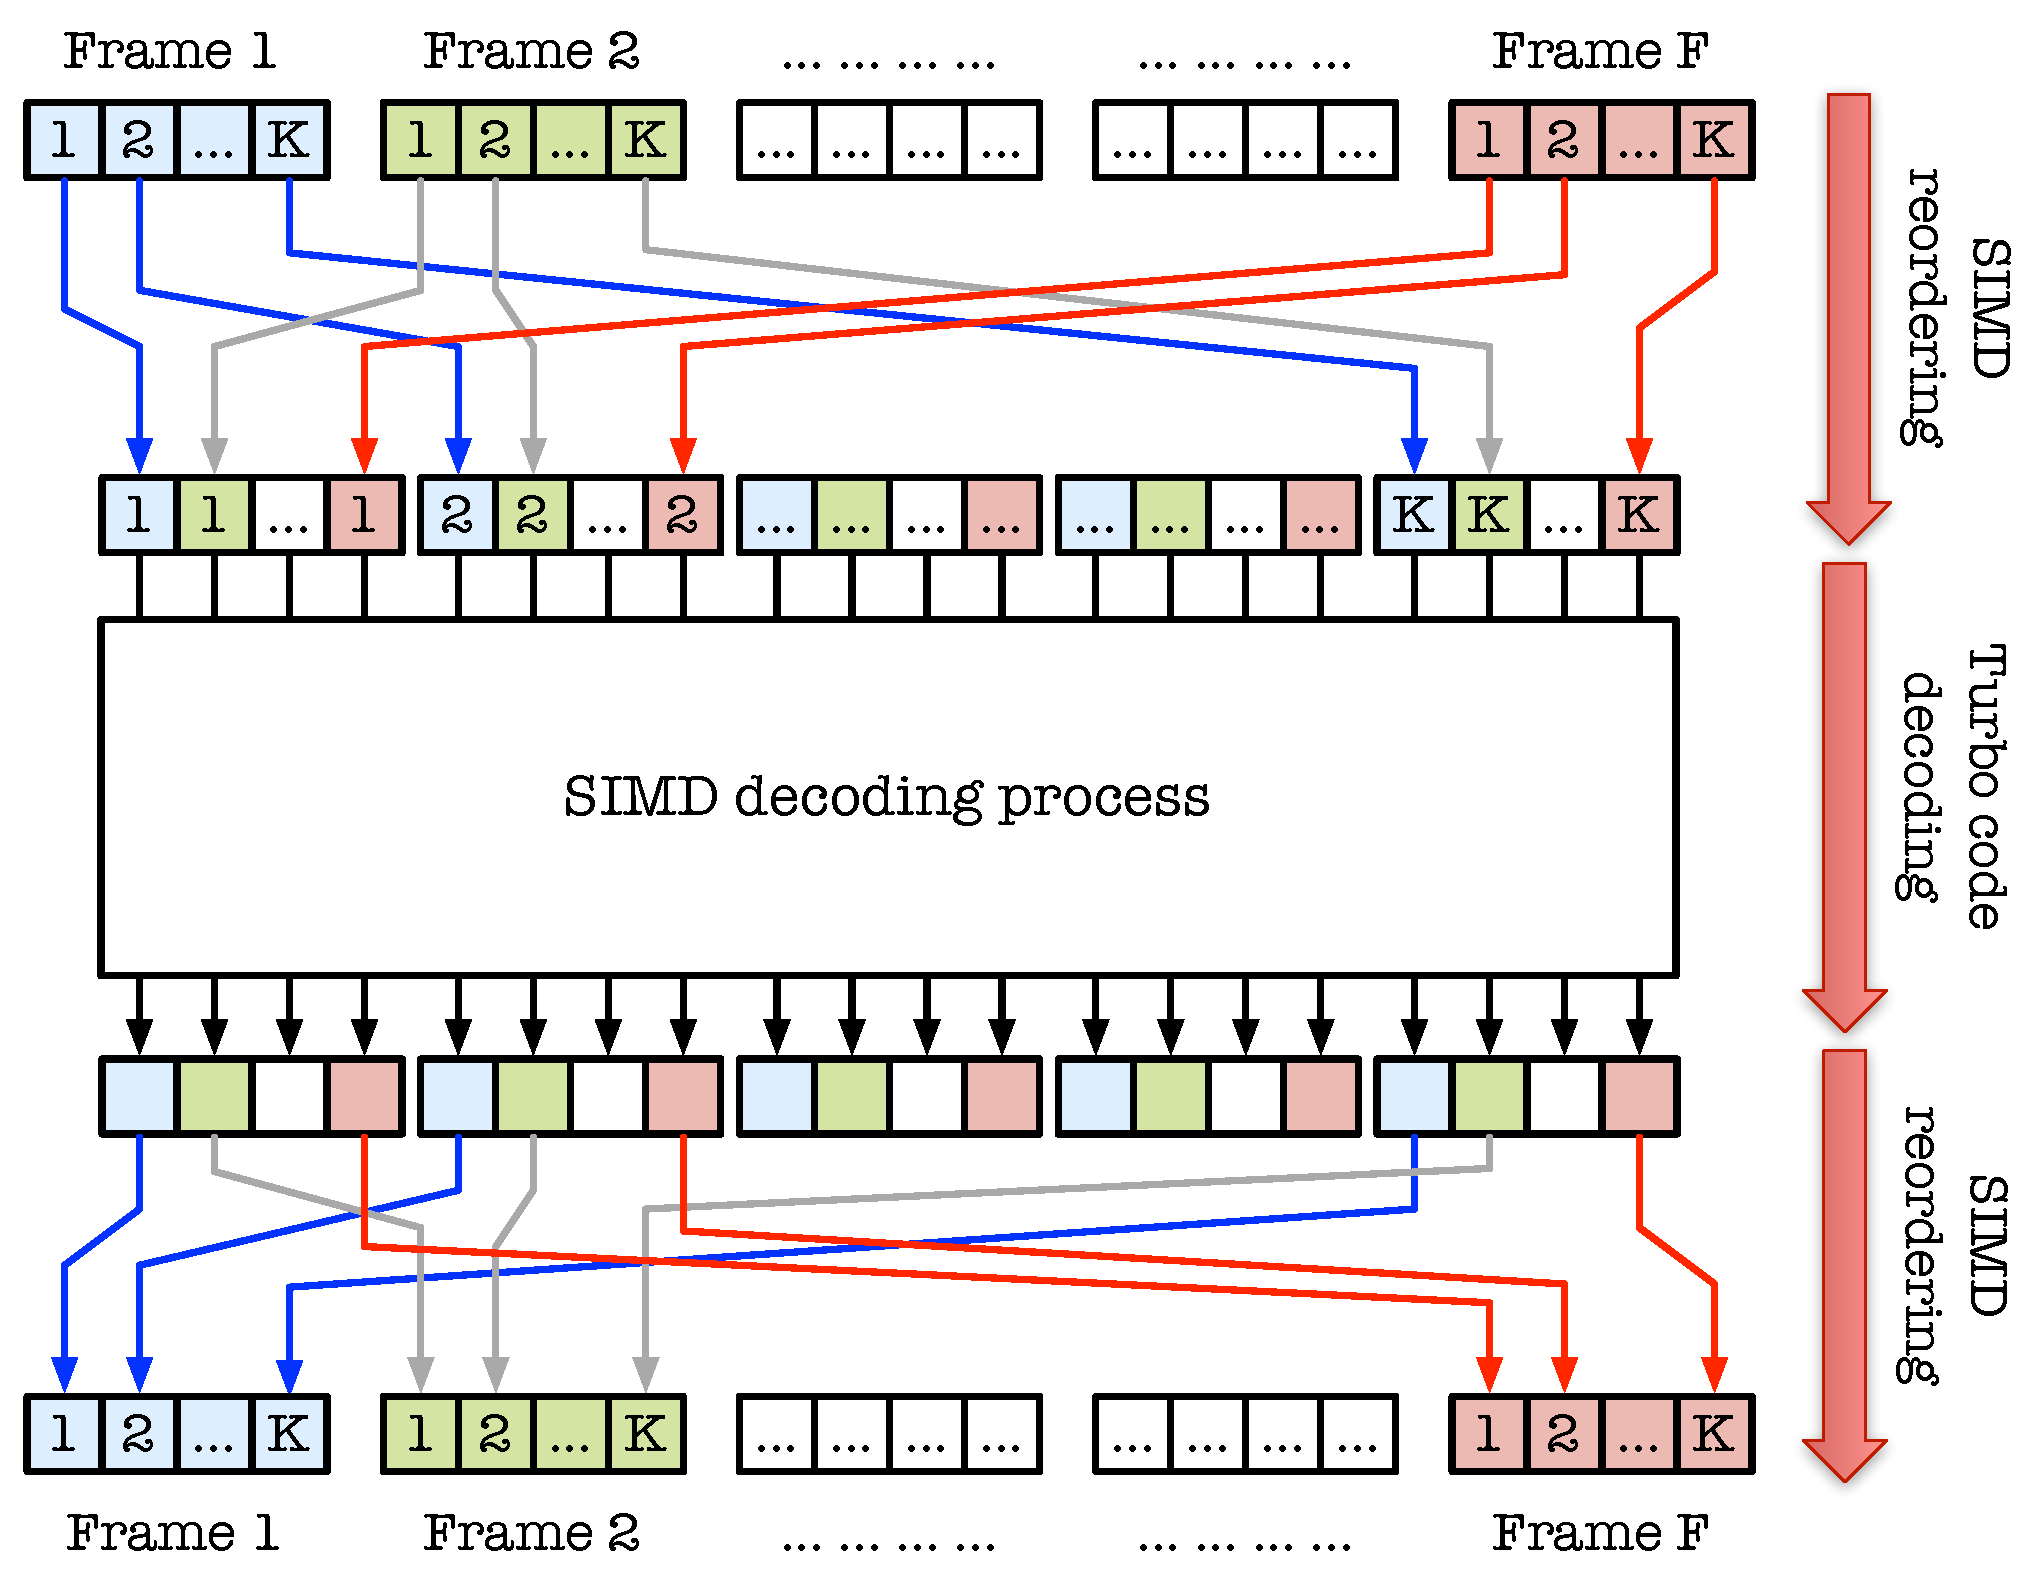
\includegraphics[width=0.70\textwidth]{turbo/reordering_process_inter_simd}
  \caption
    [Frame reordering operation before and after the turbo decoding process.]
    {Frame reordering operation before and after the decoding process. Performed
    3 times: for systematic, first and second parity information.}
  \label{fig:turbo_reordering_process_inter_simd}
\end{figure}

The contribution of this work is to propose an efficient mapping of multiple
frames on the CPU SIMD units (inter-frame strategy): the decoding of $M$ frames
is vectorized. Before the decoding process can be launched, this new approach
requires to: (a) buffer a set of $M$ frames and (b) reorder the input LLRs in
order to make the SIMDization efficient with memory aligned transactions (see
Fig.~\ref{fig:turbo_reordering_process_inter_simd}). Similarly, a
reversed-reordering step has to be performed at the end of the decoding process.
These reordering operations are expensive but they make the complete decoding
process very regular and efficient for SIMD parallelization. Moreover,
reordering is applied only once, independently of the number of decoding
iterations.

\begin{algorithm}
  \caption{Loop fusion BCJR implementation}
  \label{alg:turbo_bcjr_loop_fusion}

  % \small
  \For(// Vectorized loop){$all~frames$}
  {
    $\boldsymbol{\alpha}^0\gets \initAlpha()$

    \For(// Sequential loop){$k=1;~k<K;~k=k+1$}
    {
      $\boldsymbol{\gamma}^{k-1}\gets \computeGamma(L_{sys}^{k-1}, L_{p}^{k-1}, L_{e}^{k-1})$

      $\boldsymbol{\alpha}^k\gets \computeAlpha(\boldsymbol{\alpha}^{k-1}, \boldsymbol{\gamma}^{k-1})$
    }

    $\boldsymbol{\gamma}^{K-1}\gets \computeGamma(L_{sys}^{K-1}, L_{p}^{K-1}, L_{e}^{K-1})$

    $\boldsymbol{\beta}^{K-1}\gets \initBeta()$

    $L_e^{K-1}\gets \computeExtrinsic(\boldsymbol{\alpha}^{K-1}, \boldsymbol{\beta}^{K-1}, \boldsymbol{\gamma}^{K-1})$

    \For(// Sequential loop){$k=K-2;~k \geq 0;~k=k-1$}
    {
      $\boldsymbol{\beta}^k\gets \computeBeta(\boldsymbol{\beta}^{k+1}, \boldsymbol{\gamma}^{k})$

      $L_e^{k}\gets \computeExtrinsic(\boldsymbol{\alpha}^{k}, \boldsymbol{\beta}^k, \boldsymbol{\gamma}^{k})$
    }
  }
\end{algorithm}

In the proposed implementation, the inter-frame parallelism is used to fill the
SIMD units of the CPU cores. Algorithm~\ref{alg:turbo_bcjr} illustrates the
traditional implementation of the BCJR (used for the \emph{intra-frame}
vectorization). The inter-frame strategy makes the outer loop on the frame
parallel (through vectors). This means all computations inside this loop operate
on SIMD vectors instead of scalars, and the inner loops can be turned into
sequential loops on SIMD vectors. This gives the opportunity for memory
optimizations, through loop fusion. The initial 4 inner loops are merged into 2
loops. Algorithm~\ref{alg:turbo_bcjr_loop_fusion} presents this loop fusion
optimization. This makes possible the scalar promotion of $\beta_j$ (no longer
an array), since it can be directly reused from the CPU registers. In this
version, the SIMD are always stressed.

On a multicore processor, each core decodes $M$ frames using its own SIMD unit
and $T$ threads are activated, a total of $M\times T$ frames are therefore
decoded simultaneously with the inter-frame strategy. Theoretically, this SPMD
parallelization strategy provide an acceleration up to a factor $T$, with $T$
cores. Large memory footprint, exceeding L3 cache capacity may reduce the
effective speedup, as shown in Section~\ref{sec:eval_turbo}.

\subsection{Implementation of the decoder}
\label{sec:turbo_implem}

The presented decoder implementation is available in the \AFFECT software. The
use of \Cxx templates associated to our generic SIMD library enables the
same source code to be compiled using different formats (32-bit \verb|float|,
16-bit \verb|short|, and 8-bit \verb|char|) and different SIMD instructions
(SSE, AVX and NEON), providing possible trade-offs between SIMDization,
throughput and error-correction performance.

\subsubsection{Fixed-point representation}

Nowadays on x86 CPUs, there are large SIMD registers: SSE/NEON are 128 bits
wide and AVX are 256 bits wide. The number of elements that can be vectorized
depends on the SIMD length and on the data format:
$n_{elem} = \sizeof(SIMD) / \sizeof(data)$. So, the key for a large parallelism
is to work on short data.

As there is no floating-point support for 16-bit and 8-bit data, a fixed-point
representation is used. The AWGN channel soft information is quantized as
%follows: $y_{s,v}^k = -2^{s-1} < 2^v . y^k \pm 0.5 < 2^{s-1}$, with $y^k$
follows: $y_{s,v}^k = \Psi(2^v . y^k \pm 0.5)$, with $y^k$ the current
floating-point value from the channel, $s$ the number of bit of the quantized
number, including $v$ bits for the fractional part and the saturation function
$\Psi(x) = min(max(x, -2^{s-1} +1), 2^{s-1} -1)$. In the experiments
(cf. Fig.~\ref{plot:turbo_bfer}) $Q_{s,v}$ denotes this channel quantization.

During the turbo-decoding process, the extrinsic values grow at each iteration.
It is then necessary for internal LLRs to have a larger dynamic than the channel
information. Depending on data format, 16-bit or 8-bit, the quantization used in
the decoder is $Q_{16,3}$ or $Q_{8,2}$, respectively.

\subsubsection{Memory allocations}

The systematic information $L_{sys_N}$/$L_{sys_I}$ and the parity information
$L_{p_N}$/$L_{p_I}$  are stored in the natural domain $N$ as well as in the
interleaved domain $I$. Two extrinsic vectors are also stored: $L_{e_N}$ in $N$
and $L_{e_I}$ in $I$. Inside the BCJR decoding and per trellis section, two
$\gamma_{i}$ and eight $\alpha_{j}$ metrics are stored. Thanks to the loop
fusion optimization, the eight $\beta_j$ metrics are not stored in the global
memory. In the proposed implementation $i \in \{0,1\}$ and
$j \in \{0,1,2,3,4,5,6,7\}$. Notice that all those previously-mentioned vectors
are $K$-bit wide and are duplicated $M\times T$ times because of the inter-frame
strategy. The memory footprint in bytes is approximatively equal to:
$16 \times K \times sizeof(data) \times M \times T$.
The interleaving and deinterleaving lookup tables have been neglected in this
model.
%We did not consider the 2 lookup tables (interleaving and deinterleaving) in
%this model as they are not duplicated $M\times T$ times.

\subsubsection{Forward trellis traversal}

The objective is to reduce the number of loads/stores, performing the arithmetic
computations (\verb|add| and \verb|max|) inside registers. The max-log-MAP
algorithm only stresses the integer pipeline of the CPU. This kind of operations
takes only one cycle to execute when the latency is also very small (1 cycle
too). In contrast, a load/store can take a larger number of cycles depending on
where the current value is loaded/stored in the memory hierarchy. Using data
directly from the registers is cost-free but loading/storing it from the
L1/L2/L3 cache can take up to 30 cycles (at worst).

Per trellis section $k$, the two $\gamma_i^k$ metrics are computed from the
systematic and the parity information. These two $\gamma_i^k$ are directly
reused to compute the eight $\alpha_j^k$ metrics. Depending on the number of
bits available, the trellis traversal requires to normalize the $\alpha_j^k$
because of the accumulations along the multiple sections.  In 8-bit format, the
$\alpha_j^k$ metrics are normalized for each section: the first $\alpha_0^k$
value is subtracted to all the $\alpha_j^k$ (including $\alpha_0^k$ itself). In
the 16-bit decoder, the normalization is only applied every eight steps (like
in~\cite{Wu2013}), since there are enough bits to accumulate eight values. We
have observed in experiments that there is no performance degradation due to the
normalization process. At the end of a trellis section $k$ the two $\gamma_i^k$
and the eight normalized $\alpha_j^k$ are stored in  memory. In the next trellis
section ($k+1$) the eight previous $\alpha_j^k$ are not loaded from memory but
they are directly reused from registers to compute the $\alpha_j^{k+1}$ values.

\subsubsection{Backward trellis traversal}

Per trellis section $k$, the two $\gamma_i^k$ metrics are loaded from the
memory. These two metrics are then used to compute, on the fly, the eight
$\beta_j^k$ metrics (whenever needed the $\beta_j^k$ metrics have been
normalized like for the $\alpha_j^k$ metrics). After that, the $\alpha_j^k$
metrics are loaded from the memory. The $\alpha_j^k$, $\beta_j^k$ and
$\gamma_i^k$ metrics are used to determine the \textit{a posteriori} and the
extrinsic LLRs. In the next trellis section ($k-1$) the previous $\beta_j^k$
metrics are directly reused from registers in order to compute the next
$\beta_j^{k-1}$ values. The $\beta_j^k$ metrics are then never stored in the
memory.

\section{LDPC Decoders}

\begin{itemize}
  \item \xmark~section très incomplète
  \item \xmark~on pourrait parler de la technique utilisée pour avoir des
    décodeurs BP génériques (avec des illustrations de code, ça repose sur du
    C++17), décodeurs séquentiels ou vectorisation inter-frame
  \item \xmark~peut être mettre quelques petits résultats en terme de débit et
    latence ici plutôt que dans la section évaluation puisqu'il n'y a pas de
    publications
\end{itemize}

% LDPC codes is a family of channel codes that is well spread in current digital
% communication systems. They have been chosen in many communication standards
% (Wifi, WiMAX, DVB-S2, 10Gbps Ethernet, etc.). They were also selected for the
% future 5G standard data transport.

% In this section the Min-Sum decoder for LDPC codes is presented. As shown in
% Figure~\ref{fig:ldpc}, an LDPC code can be represented in the form of a Tanner
% graph. The circles, denoted as variable nodes, represent the LLRs (the noisy
% estimation of the bits in the received frames). The squares, denoted as parity
% check nodes, represent the parity constraints that the variable nodes have to
% verify. For instance, the check node $a$ ($CN_a$) is connected to the variable
% nodes $1$, $4$, $5$, $7$ and $8$ ($VN_1, VN_4, VN_5, VN_7, VN_8$). It means that
% the corresponding bits $U_1, U_4, U_5, U_7, U_8$ have to respect a parity
% constraint: $U_1 \oplus U_4 \oplus U_5 \oplus U_7 \oplus U_8 = 0$. A codeword is
% valid only if it respects all the parity constraints defined by the check nodes.
% The LDPC code can be also represented by a \textit{parity check matrix}:
% { \begin{equation*}
% H =
% \begin{bmatrix}
%   1&0&0&1&1&0&1&1\\
%   0&1&1&0&0&1&1&0\\
%   1&0&1&0&0&1&0&1\\
%   0&1&0&1&1&0&1&0
% \end{bmatrix}.
% \end{equation*}
% }
% The Min-Sum decoder is an iterative message passing algorithm based on the
% Tanner graph representation. Probabilistic messages ($M$) are exchanged between
% the variable nodes and check nodes iteratively. Variable nodes and check nodes
% apply an \textit{update rule} to compute the outgoing messages from the incoming
% messages. In this section, the Min-Sum update rule is considered as well as an
% horizontal layered scheduling. The original version of the Min-Sum algorithm
% works on floating-point values, but it has been shown that fixed-point
% simplifications have very similar decoding performance. Moreover, a fixed-point
% representation enables to pack more elements into SIMD registers.

\begin{listing}[htp]
  \inputminted[frame=lines,linenos]{C++}{main/chapter3/src/ldpc/bp_min_sum_simd.cpp}
  \caption{LDPC decoder implementation with \MIPP.}
  \label{lst:vec_ldpc_bp_min_sum_simd}
\end{listing}

\begin{table}[htp]
  % \tabcolsep=6pt
  \centering
  \caption{LDPC decoder speedups with \MIPP.}
  \label{tab:vec_ldpc_speedup}
  % {\small
  \begin{tabular}{r| r r r}
                      & \textbf{NEON} & \textbf{SSE} & \textbf{AVX}  \\ \hline \hline
  \textbf{SIMD size}  & 8             & 8            & 16            \\ %\hline
  \textbf{T/P} (Mb/s) & 8.3           & 30.3         & 53.2          \\ %\hline
  \textbf{Speedup}    & $\times 9.7$  & $\times 8.8$ & $\times 15.2$ \\
  \end{tabular}
  % }
\end{table}

Listing~\ref{lst:vec_ldpc_bp_min_sum_simd} shows a 16-bit fixed-point LDPC
decoder. This decoder works on several frames at once. Each element of the SIMD
registers corresponds to an element of a specific frame. This approach is called
the \textit{inter-frame} vectorization. This strategy maximizes decoder
throughput at the expense of latency. Notice that the data type can be switched
from \verb|int16_t| to \verb|int8_t|, \verb|int32_t|, \verb|float| or
\verb|double|. This \MIPP feature is important for digital communication:
adapting the data type without changing the source code enables to address
varying constraints with a single source code. Table~\ref{tab:vec_ldpc_speedup}
presents speedups obtained with \MIPP. Ten iterations are performed and a stop
criterion was implemented for the tests based on parity check constraints (not
shown in Listing~\ref{lst:vec_ldpc_bp_min_sum_simd}). The $H$ matrix comes from
the IEEE 802.3an standard (10Gbps Ethernet). Speedups are close to the SIMD
width. In NEON and SSE they even exceed it. Such result can be explained by an
optimized memory management compared to the sequential version of the code.

\section{SCMA Demodulators}
\label{sec:opt_scma}

Besides methodical improvements of the MPA such as log-MPA, hardware oriented
improvements are important to take full benefit of C-RAN servers capabilities.
Since MPA and log-MPA are control heavy algorithms, mishandling of data can
induce huge performance losses. This section explores how MPA can be
reformulated: 1) to improve data locality in cache and to reduce cache misses
and branch mispredictions 2) to reorder the data paths in order to help
exploiting data-level parallelism at each step of the MPA and log-MPA algorithms
and 3) to exploit approximated modeling of additive white Gaussian noise in
order to eliminate exponential calculations and to drastically reduce the number
of instructions for SSE, NEON, AVX and KNCI ISAs.

\subsection{Flattening Matrices to Reduce Cache Misses and Branch Misses}
\label{sec:opt_scma_flattening}

Considering \eqref{eq:scma_6} and \eqref{eq:scma_7}, there are 64 calculations
of distances and probabilities for each resource (256 for all resources). Using
a multidimensional array ($4\times4\times4$) should be avoided, because it
typically causes bad data locality, which leads to an increased number of cache
misses. These misses negatively affect the throughput, and this is significant,
since this process must be repeated in the decoder for each received 12-bit
block of data. Flattening a $d$-dimensional array to a vector using
\eqref{eq:scma_17} is appropriate to prevent cache misses and improve the
spatial locality of data. This is done with the help of an index defined as:
\begin{equation}
  \label{eq:scma_17}
  index = \sum\limits_{i=1}^d\Bigg( \prod\limits_{j=i+1}^d N_j \Bigg)n_i.
\end{equation}
Where $N_j$ is the size of the $j^{th}$ dimension of the array and $n_i$ is the
location of a target element in that dimension. Improving data locality with
a stride of a single floating-point number in each element makes it easier for
the processor to have aligned and contiguous accesses to the memory through SIMD
ISA. Utilizing SIMD instructions helps to reduce the total number of
mispredicted branches in the algorithm. Contiguous accesses to the L1 cache are
performed by chunks of 128-bit, 256-bit or 512-bit. It reduces the number of
iterations in the \verb|for|-loops and consequently it reduces the number of
branches. On the other hand, for a vector of sixty four 32-bit floating-point
numbers, 64 iterations are needed in the scalar mode, while only 16, 8 or 4
iterations are required in the vectorized modes using respectively SSE (or
NEON), AVX or KNCI ISAs.

\subsection{Adapting the Algorithms to Improve Data-Level Parallelism}
\label{sec:opt_scma_adapting_algorithms}

SSE, NEON, AVX and KNCI ISAs handle SIMD operations. KNCI and AVX use 512-bit
and 256-bit registers, while SSE and NEON use 128-bit registers. For instance,
an AVX operation can process eight 32-bit floating-point numbers simultaneously.
The AVX instructions also provide high-performance loads and stores to the cache
memory due to data vectorization. Flattening matrices to vectors is a
prerequisite to enable AVX contiguous accesses to the memory. Vectorized
instructions such as AVX are accessible in C++ through intrinsic functions. An
intrinsic is a function that directly maps to an assembly instructions (for some
rare exceptions it can be more than one instruction). Nowadays, AVX units use
sixteen 256-bit YMM registers and a 32-bit MXCSR control register to handle
vectors of eight 32-bit or four 64-bit floating-point numbers. The AVX ISA
allows to perform SSE instructions using the lower 128-bit lane of the YMM
registers. For MPA, the SIMD instructions are used to 1) compute the complex
norm $||.||$ in \eqref{eq:scma_5} and \eqref{eq:scma_6}, 2) calculate the
exponentials in \eqref{eq:scma_7}, 3) perform users to resources messaging and
final guesses at each user.

\subsubsection{SIMD Computation of Complex Norms}

\begin{figure}[htp]
  \centering
  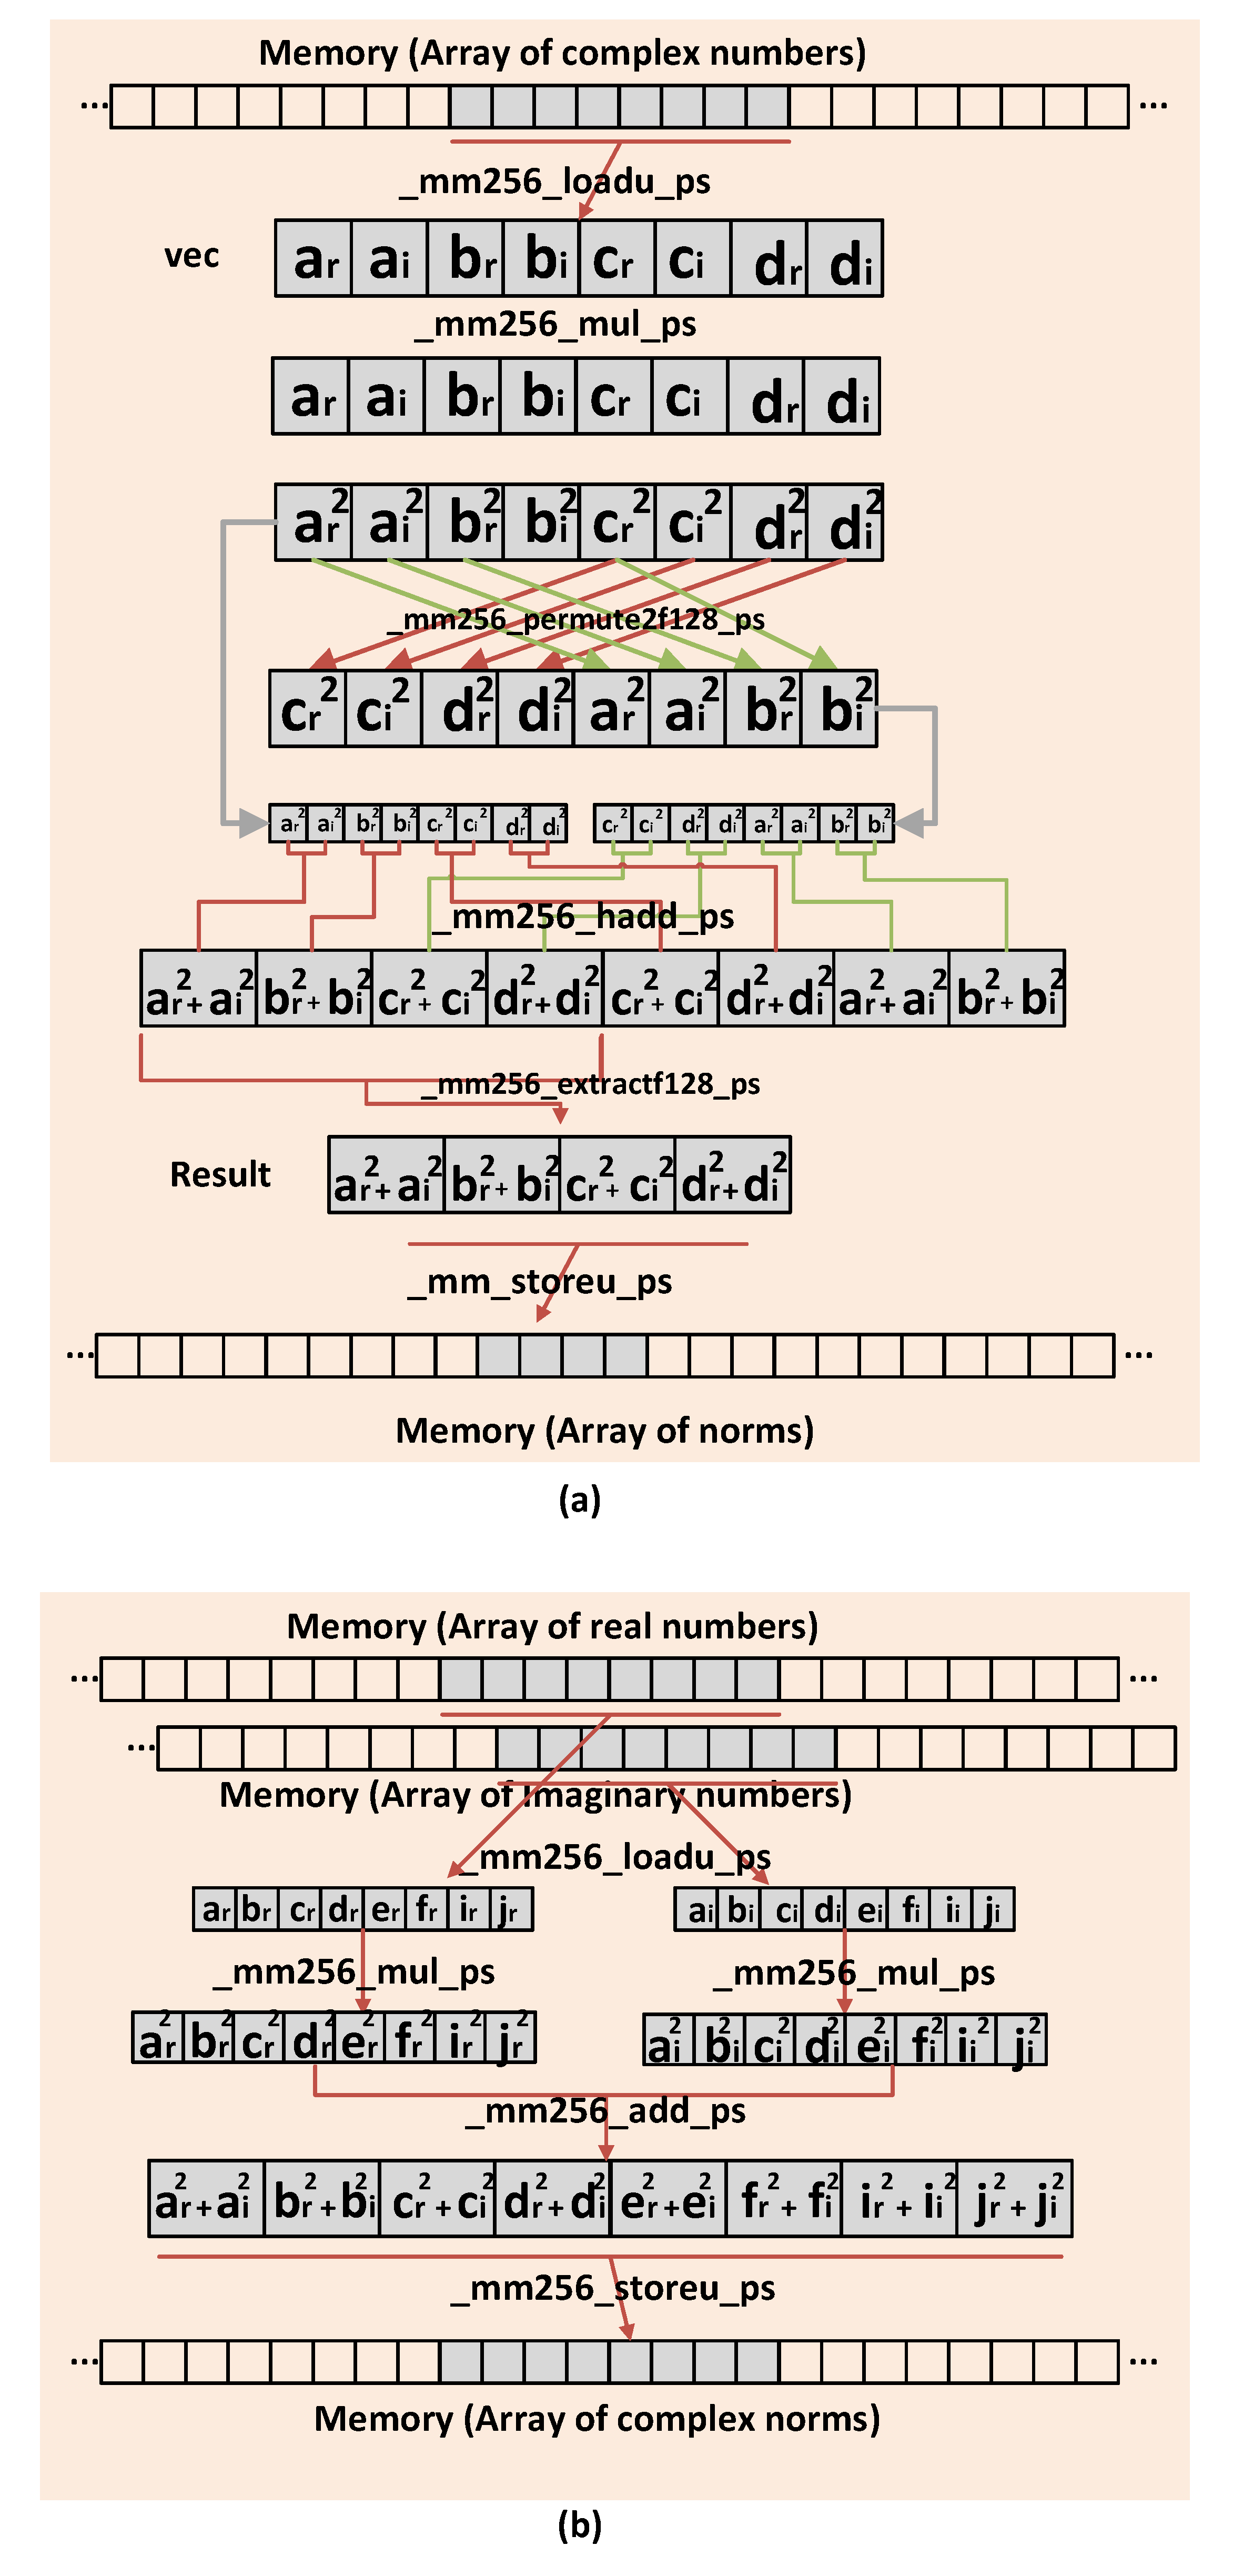
\includegraphics[width=0.70\linewidth]{scma/simd_norm/simd_norm}
  \caption
    [MPA complex norm AVX algorithm using AoS and SoA.]
    {MPA complex norm AVX algorithm using
     a) Array of Structures (AoS),
     b) Structure of Arrays (SoA).}
  \label{fig:scma_simd_norm}
\end{figure}

Equations~\eqref{eq:scma_5} and \eqref{eq:scma_6} use a complex norm function
$||.||$, it can be optimized by using SIMD instructions. There are two ways to
perform this computation: Fig.~\ref{fig:scma_simd_norm}a depicts how to
implement the norm function using an Array of Structures (AoS) for complex
numbers. In this method, the complex numbers are represented as two consecutive
floating-point numbers. The implementation with AoS uses six intrinsic
functions: one load (\verb|_mm256_loadu_ps|), one store
(\verb|_mm256_storeu_ps|), one multiplication (\verb|_mm256_mul_ps|), one
permutation of the lanes (\verb|_mm256_permute2f128_ps|), one horizontal
addition (\verb|_mm256_hadd_ps|) and one extraction of the highest lane of the
AVX register (\verb|_mm256_extractf128_ps|). Fig.~\ref{fig:scma_simd_norm}b
sketches the computation of the complex norm using a Structure of Array (SoA)
data layout. This implementation also uses six intrinsic functions: two loads
(\verb|_mm256_loadu_ps|), one store (\verb|_mm256_storeu_ps|), two standard
multiplications (\verb|_mm256_mul_ps|), one addition (\verb|_mm256_add_ps|).

Our experiments demonstrated that these two methods have similar performances,
however we used the Structure of Arrays (SoA) since it is 1) easier to port for
the ISAs that lack from shuffle instructions and 2) trivial to extend for
different register lengths.

\subsubsection{SIMD Computation of Exponential}

To speedup the computational time of the exponentials used in \eqref{eq:scma_7},
the MIPP wrapper~\cite{Cassagne2018} has been used. MIPP proposes a vectorized
implementation of the exponential based on a series expansion. Many intrinsic
functions are encapsulated to compute the exponential. MIPP also allows to write
portable intrinsic codes. A single SIMD code is written for multiple ISAs such
as SSE, NEON, AVX, AVX-512 and KNCI thanks to the meta-programming techniques.

\begin{figure}[htp]
  \centering
  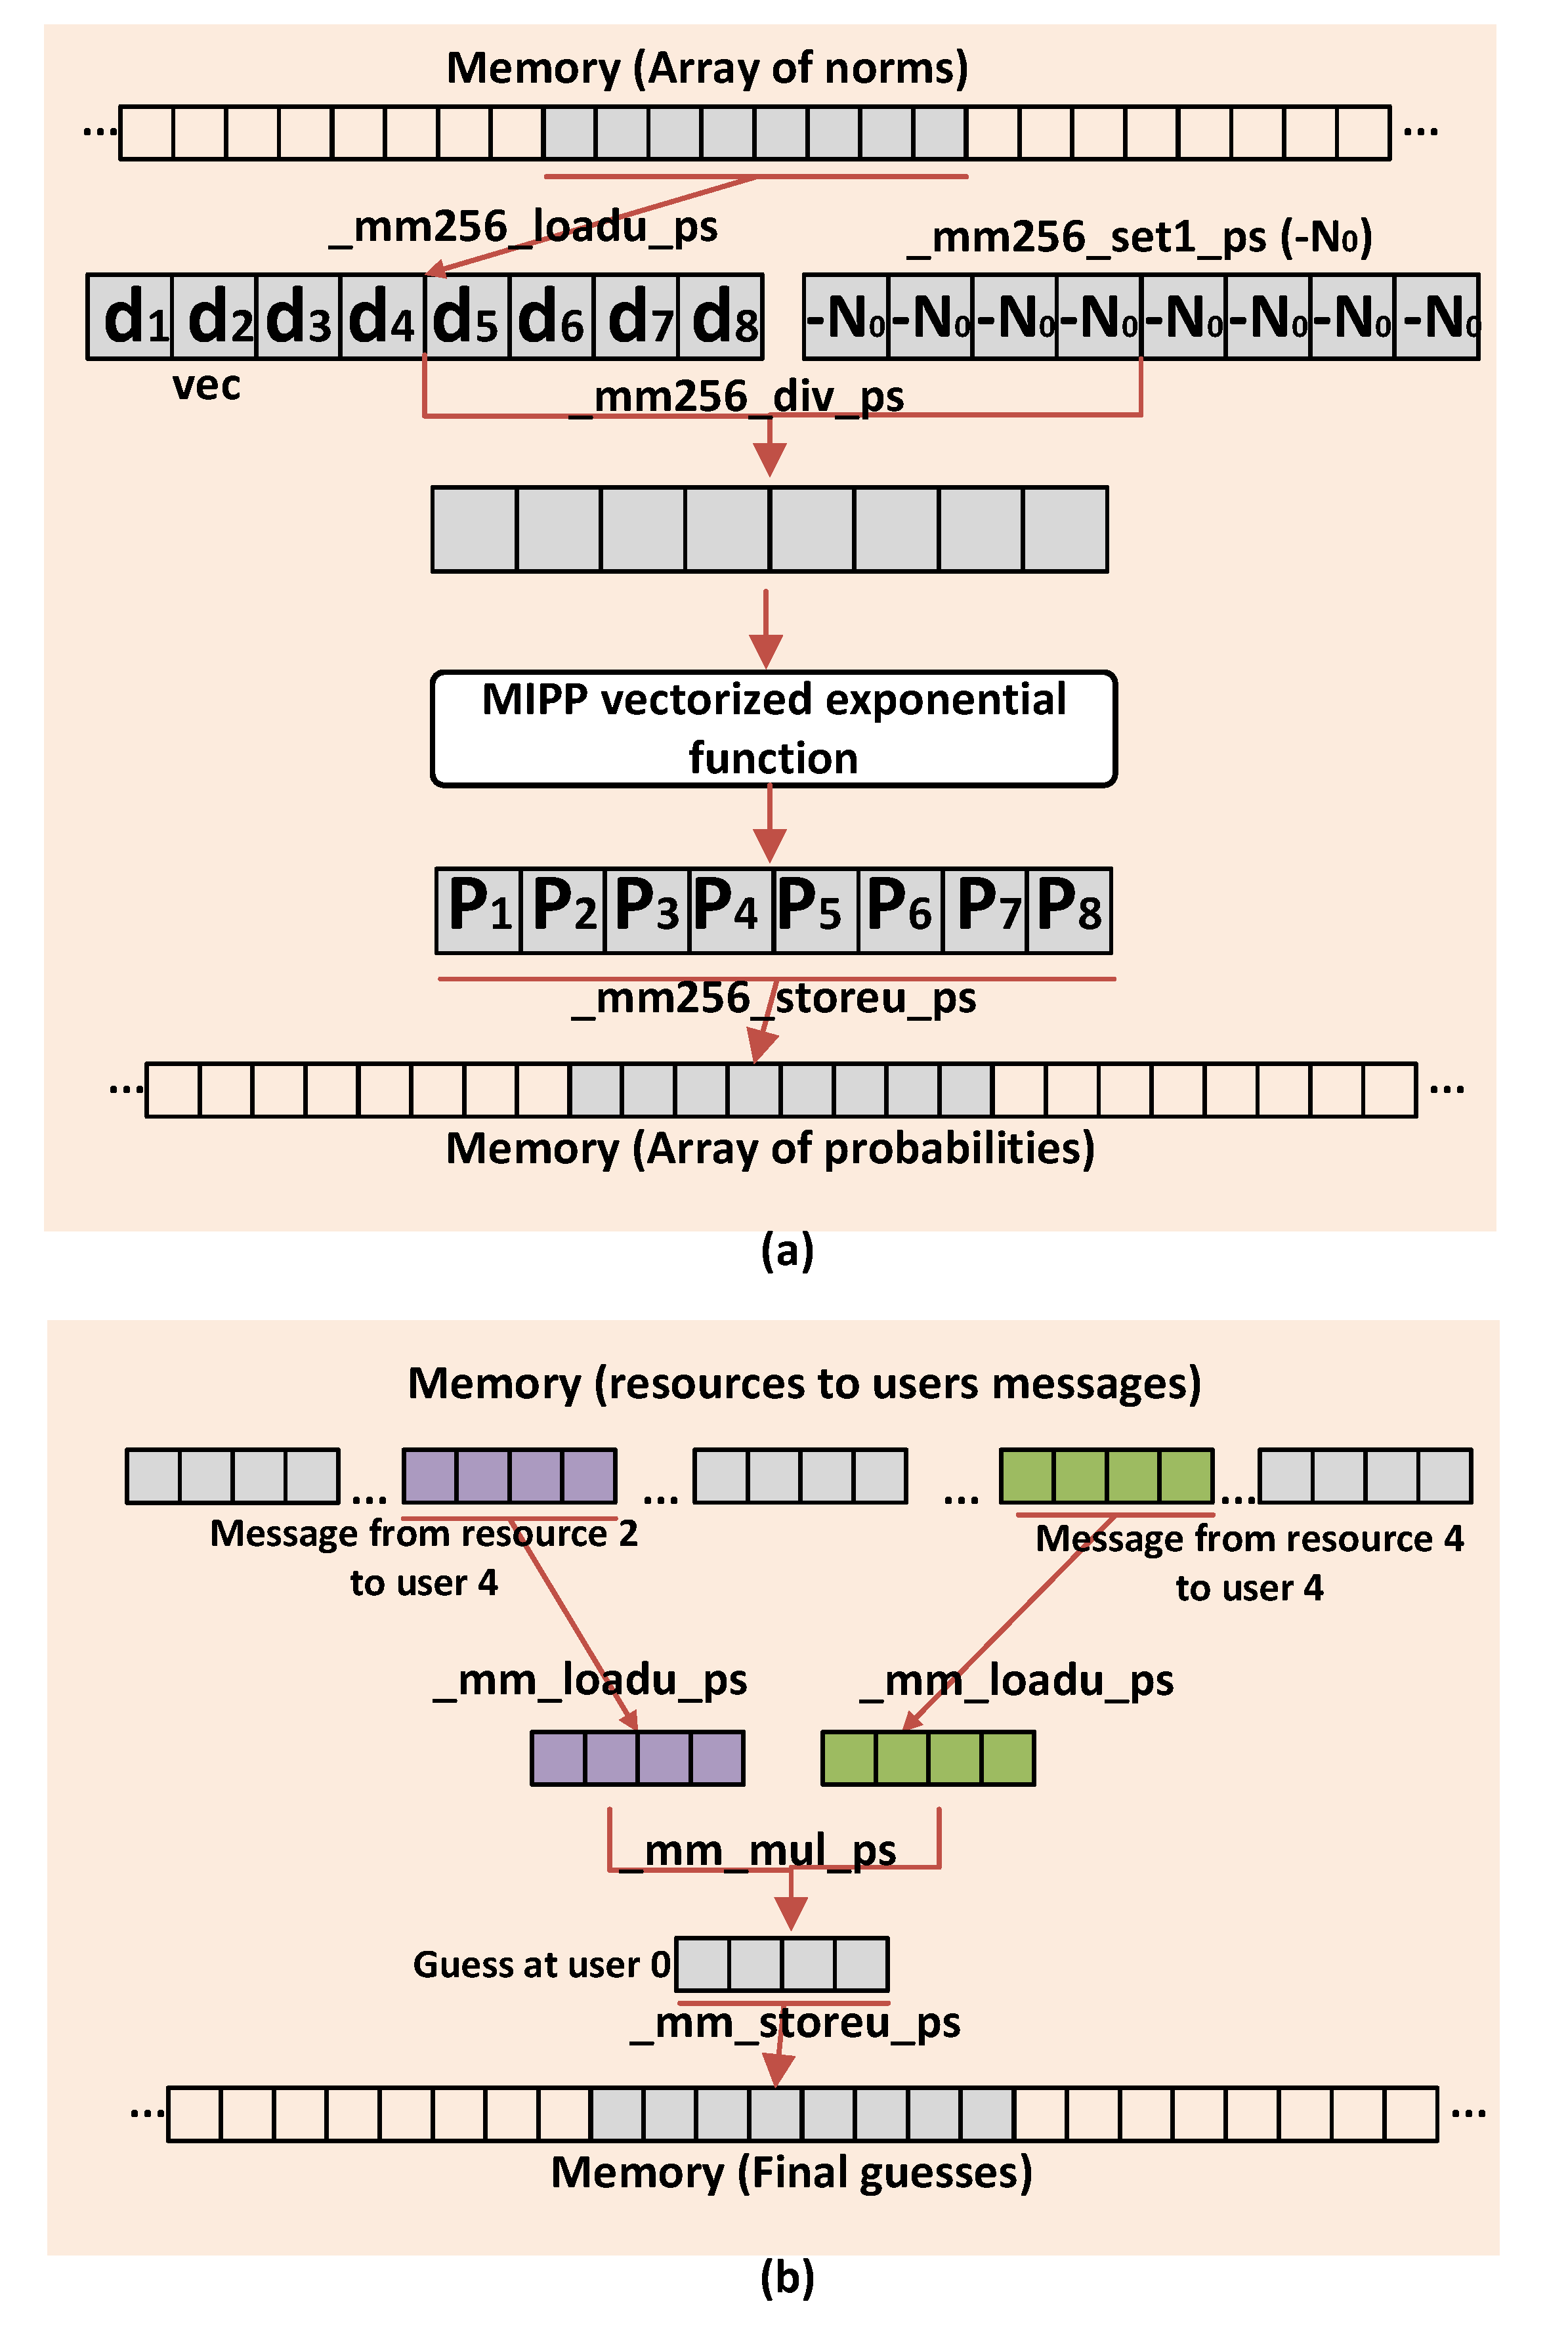
\includegraphics[width=0.70\linewidth]{scma/simd_exp_mul/simd_exp_mul}
  \caption
    [MPA vectorized Exponentials ($N_0 = 2\sigma^2$).]
    {a) Vectorized Exponentials ($N_0 = 2\sigma^2$),
     b) Vectorized calculation of final guess at user 4.}
  \label{fig:scma_simd_exp_mul}
\end{figure}

The flattened complex and normalized numbers are calculated as shown in
Fig.~\ref{fig:scma_simd_norm}a and Fig.~\ref{fig:scma_simd_norm}b to produce the
preliminary values used to compute the probabilities.
Fig.~\ref{fig:scma_simd_exp_mul}a illustrates the full process on a vector of
eight floating-point numbers. First the values are loaded into the YMM
registers, then they are multiplied by $-1/2\sigma^2$ and finally the
exponential function is performed according to \eqref{eq:scma_7}.

\subsubsection{Exponential Approximation: Estimated-MPA (E-MPA)}

\eqref{eq:scma_19} can be used as a systematic replacement to the vectorized
exponential MIPP function used in Fig.~\ref{fig:scma_simd_exp_mul}a. It reduces
the overall number of instructions to three intrinsic functions: two
multiplications (\verb|_mm256_mul_ps|) and one addition (\verb|_mm256_add_ps|).

\subsubsection{SIMD Message Passing}

Some remaining parts of the MPA can be vectorized too. Especially, the guess
swaps and the computation of the final guesses at each user node can be
vectorized using SSE instructions. Fig.~\ref{fig:scma_simd_exp_mul}b shows the
computation of final guesses for user 4. There are four messages from a resource
to a user containing the probabilities of four different codewords, which are
the elements of the SSE vectors. According to Fig.~\ref{fig:scma_simd_exp_mul}b
these vectors of probabilities are loaded into SSE, NEON or the lowest lane of
the AVX registers.

% \subsection{Accuracy of Floating-point Computations and Other Traditional Optimization}
\subsubsection{Accuracy of Floating-point Computations}
\label{sec:opt_scma_float}

The finite precision of floating-point calculations induces losses in the
results. Thus, technical standards such as IEEE 754 define rounding rules,
precision of calculations, exception handling and underflow behavior. However,
the MPA delivers approaching bit error rate results with less precise
floating-point models. For instance, in the GNU compiler, \verb|-Ofast| is a
high-level compiler option which includes fast math libraries to handle
floating-point calculations (\verb|-ffast-math|). The compiler uses various
mathematical simplifications as explained in~\cite{Gccfp2018} and uses
approximated libraries for the division and the square root functions. The
compiler also forces the value to zero in the case of an underflow. Using
\verb|-Ofast| can improve the throughput of the MPA algorithm as will be shown
in Section~\ref{sec:eval_scma}.

In this work, other well-known optimization techniques, such as loops unrolling,
using references instead of pointers, avoiding type conversions, preferring
prefixed operators, and functions inlining have been used to enhance the
throughput of the various message passing algorithms.

\section{Discussion}

\begin{itemize}
  \item \xmark~le temps d’exécution d’une tâche peut varier entre quelques
    microsecondes et quelques milliseconde -> faible latence -> adapté à la
    vectorisation
  \item \xmark~rappeller les optimisations clefs (quantification, memory layout
    adapté, vecto, ...)
  \item \xmark~inter-/intra vectorisation, point de vue
  \item \xmark~faiblesses des architectures CPU actuelles, comment on pourrait
    les améliorer pour ce type d'algos
  \item \xmark~optimisations non implémentées qui pourraient être bénéfiques
    (mixed-precision, bit packing à gogo)
\end{itemize}